% !TEX program = pdflatex
% University of Malakand Thesis Style (adapted)
\documentclass[12pt, a4paper, oneside]{book}

% ===== PACKAGES =====
\usepackage[utf8]{inputenc}
\usepackage[T1]{fontenc}
% Font: The university guideline asks for Times New Roman. MiKTeX installs vary; missing font
% packages can trigger interactive prompts. We prefer "compile-first" fallbacks:
% 1) TeX Gyre Termes (Times-like, usually light on dependencies)
% 2) newtx (Times-like, but may require extra packages like xpatch)
% 3) Latin Modern (always available)
\IfFileExists{tgtermes.sty}{%
  \usepackage{tgtermes}%
  \IfFileExists{newtxmath.sty}{\usepackage{newtxmath}}{}%
}{%
  \IfFileExists{newtxtext.sty}{%
    \IfFileExists{xpatch.sty}{%
      \usepackage{newtxtext}%
      \usepackage{newtxmath}%
    }{%
      \usepackage{lmodern}%
      \typeout{WARNING: newtxtext found but xpatch missing. Using Latin Modern. Install 'xpatch' (and newtx deps) for Times-like font.}%
    }%
  }{%
    \usepackage{lmodern}%
    \typeout{WARNING: Times-like font packages not found. Using Latin Modern. For Times, install 'tex-gyre' or 'newtx'.}%
  }%
}
\usepackage{geometry}          % Margins
\usepackage{xcolor}            % Colors (kept minimal; used in plots/tables)
\usepackage{tikz}              % Diagrams
\usetikzlibrary{positioning,arrows.meta}
\usepackage{pgfplots}          % Charts
\pgfplotsset{compat=1.18}
\usepackage{fancyhdr}          % Footer page numbers (bottom-right)
\usepackage{multicol}          % Two-column lists/sections
\usepackage{amsmath, amssymb}  % Math
\usepackage{graphicx}          % Images
\usepackage{booktabs}          % Tables
\usepackage{array}             % Table columns
\usepackage{colortbl}          % Table cell colors
\usepackage{setspace}          % 1.5 line spacing
\usepackage{microtype}         % Typography
\usepackage{hyperref}          % Links
\usepackage{bookmark}          % PDF bookmarks

% ===== MARGINS (University of Malakand) =====
% A4: left 1.5 inch, other sides 1 inch
\geometry{
  a4paper,
  left=1.5in,
  right=1in,
  top=1in,
  bottom=1in,
  includeheadfoot
}

% ===== COLORS (Minimal) =====
\definecolor{DeepObsidian}{HTML}{111111}
\definecolor{LightGray}{gray}{0.95}
\definecolor{AccentBlue}{HTML}{0B5394}
% Backward-compatible names used by existing figures/plots.
\definecolor{CyberCyan}{HTML}{0B5394}
\definecolor{ElectricIndigo}{HTML}{3C78D8}

% ===== TYPOGRAPHY =====
\microtypesetup{protrusion=true, expansion=true}
\renewcommand{\familydefault}{\rmdefault}

% ===== PAGE NUMBERS (bottom-right, 3/4" from bottom) =====
\pagestyle{fancy}
\fancyhf{}
\renewcommand{\headrulewidth}{0pt}
\renewcommand{\footrulewidth}{0pt}
\fancyfoot[R]{\thepage}
\setlength{\footskip}{0.75in}
\fancypagestyle{plain}{%
  \fancyhf{}
  \renewcommand{\headrulewidth}{0pt}
  \fancyfoot[R]{\thepage}
}

% ===== SIMPLE BOX (for highlights) =====
\newenvironment{keyinsight}{%
  \begin{center}\begin{tabular}{|p{0.92\textwidth}|}\hline\small
}{%
  \\\hline\end{tabular}\end{center}
}

% ===== HYPERREF =====
\hypersetup{
  colorlinks=true,
  linkcolor=AccentBlue,
  urlcolor=AccentBlue,
  citecolor=AccentBlue
}

% ===== CUSTOM COMMANDS =====
\newcommand{\thesistitle}{Cardiovascular Disease Prediction Using Machine Learning}
\newcommand{\thesisauthor}{Sajjad Alam}
\newcommand{\thesisdegree}{Bachelor of Science (Statistics)}
\newcommand{\thesisdept}{Department of Statistics}
\newcommand{\thesisuni}{University of Malakand}
\newcommand{\thesisyear}{2026}

% ===== CHAPTER STYLE =====
% Keep default book style for strict university formatting.

% ===== DOCUMENT =====
\begin{document}
\onehalfspacing

% ---- FRONTMATTER (Roman numerals) ----
\frontmatter

% ----- TITLE PAGE (not numbered) -----
\begin{titlepage}
  \thispagestyle{empty}
  \begin{center}
    {\bfseries\MakeUppercase{Thesis}\par}
    \vspace{18pt}
    {\bfseries\MakeUppercase{\thesistitle}\par}
    \vspace{18pt}
    A thesis submitted in partial fulfillment of the requirements for the degree of\par
    \vspace{10pt}
    {\bfseries \thesisdegree\par}
    \vspace{14pt}
    {\bfseries By\par}
    \vspace{10pt}
    {\bfseries\MakeUppercase{\thesisauthor}\par}
    \vspace{18pt}
    \thesisdept\par
    \vspace{6pt}
    \thesisuni\par
    \vspace{18pt}
    {\bfseries\MakeUppercase{\thesisyear}\par}
  \end{center}
\end{titlepage}

% Start roman page numbering at ii after the title page.
\pagenumbering{roman}
\setcounter{page}{2}

% ----- DECLARATION -----
\chapter*{Declaration}
\addcontentsline{toc}{chapter}{Declaration}
I, \thesisauthor, hereby declare that this thesis titled ``\thesistitle'' is my own work and has not been submitted previously for any other degree or professional qualification.
\par\bigskip
Signature:\dotfill\par
Date:\dotfill

% ----- PLAGIARISM UNDERTAKING -----
\chapter*{Plagiarism Undertaking}
\addcontentsline{toc}{chapter}{Plagiarism Undertaking}
I solemnly declare that the research work presented in this thesis is my own work. Any material used from other sources has been properly acknowledged and cited.
\par\bigskip
Signature:\dotfill\par
Date:\dotfill

% ----- SUBMISSION AUTHORIZATION CERTIFICATE -----
\chapter*{Submission Authorization Certificate (For Evaluation)}
\addcontentsline{toc}{chapter}{Submission Authorization Certificate}
Certified that the thesis of \thesisauthor\ entitled ``\thesistitle'' has been reviewed in final form and permission is granted to submit it to \thesisuni\ for evaluation.
\par\bigskip
Supervisor:\dotfill\par
Co-supervisor (if any):\dotfill\par
Chairman:\dotfill

% ----- APPROVAL CERTIFICATE -----
\chapter*{Approval Certificate (For the Award of Degree)}
\addcontentsline{toc}{chapter}{Approval Certificate}
It is certified that the work contained in this thesis entitled ``\thesistitle'' was carried out by \thesisauthor\ under supervision and is adequate in scope and quality for the award of the degree.
\par\bigskip
Supervisor:\dotfill\par
Co-supervisor (if any):\dotfill\par
External Examiner:\dotfill\par
Chairman:\dotfill

% ----- DEDICATION -----
\chapter*{Dedication}
\addcontentsline{toc}{chapter}{Dedication}
\begin{center}
\emph{(Write your dedication here.)}
\end{center}

% ----- ACKNOWLEDGMENTS -----
\chapter*{Acknowledgments}
\addcontentsline{toc}{chapter}{Acknowledgments}
I would like to thank my supervisor, teachers, and family for their guidance and support during this research. I also acknowledge the open-source community for providing high-quality machine learning tools.

% ----- TABLE OF CONTENTS -----
\tableofcontents
\listoffigures
\listoftables

% ----- LIST OF ABBREVIATIONS -----
\chapter*{List of Abbreviations}
\addcontentsline{toc}{chapter}{List of Abbreviations}
\begin{multicols}{2}
\begin{itemize}
\item CVD: Cardiovascular disease
\item BMI: Body mass index
\item ROC: Receiver operating characteristic
\item AUC: Area under the curve
\item SHAP: SHapley Additive exPlanations
\end{itemize}
\end{multicols}

% ----- LIST OF PUBLICATIONS (optional) -----
\chapter*{List of Publications}
\addcontentsline{toc}{chapter}{List of Publications}
\emph{(If any, list your publications here.)}

% ----- ABSTRACT -----
\chapter*{Abstract}
\addcontentsline{toc}{chapter}{Abstract}
This thesis develops a practical machine learning system for predicting cardiovascular disease risk from routinely collected health attributes. Using a structured cardiovascular dataset containing demographic, clinical, and lifestyle features, multiple model families are compared (Logistic Regression, SVM, Random Forest, Neural Network, and gradient boosting). The best-performing models are deployed behind a FastAPI service with a user-friendly web interface. The system returns a probability score, a thresholded decision, and explainability information (SHAP) to highlight key drivers behind each prediction.

% ===== MAINMATTER (Arabic numerals) =====
\mainmatter
\pagenumbering{arabic}

% ===== THESIS CONTENT (from r1.docx) =====
\chapter{INTRODUCTION}

\section{Background of the Study}

Cardiovascular disease (CVD) remains a major cause of mortality globally and represents a substantial public health burden. Millions of people lose their lives every year due to heart-related diseases like heart failure, coronary artery disease, and stroke, health reports worldwide have claimed. These diseases are often linked with lifestyle risk factors such as an unhealthy diet, inadequate physical activity, smoking, and diabetes, high blood pressure and obesity. It is important Because it can be a very deadly disease and early detection of the disease in order to improve, implementation of necessary treatment options.

Traditional medical diagnosis relies heavily on physicians’ experience, laboratory tests, and clinical guidelines. While these methods are effective, they may sometimes fail to capture complex patterns and hidden relationships within medical data. With the increasing availability of healthcare data and advancements in computing technologies, machine learning has emerged as a powerful approach for analyzing large medical datasets and assisting in disease prediction.

Machine learning algorithms are capable of learning patterns from historical data and making predictions on new, unseen data. In the healthcare domain, these techniques can assist doctors in identifying high-risk patients and supporting early diagnosis. Machine learning models such as Logistic Regression, Random Forest, Support Vector Machine (SVM), and Gradient Boosting have been widely used in medical research for disease prediction tasks.

The cardiovascular disease dataset used in this research contains various medical attributes such as age, gender, blood pressure, cholesterol levels, glucose levels, smoking habits, alcohol consumption, and physical activity. By analyzing these features, machine learning models can identify patterns that may indicate whether a person is likely to develop cardiovascular disease.

The application of machine learning in healthcare has the potential to improve diagnostic accuracy, reduce healthcare costs, and provide decision support to medical professionals. Therefore, developing a reliable cardiovascular disease prediction model is an important research area in modern healthcare analytics.

\section{Problem Statement}

Despite advancements in medical science, cardiovascular disease remains a major cause of mortality across the globe. Early detection and prevention are essential for reducing the impact of heart-related diseases. However, traditional diagnostic methods often depend on manual interpretation of clinical data, which can be time-consuming and prone to human error.

Medical datasets usually contain a large number of variables and complex relationships between them. Traditional statistical models may struggle to accurately identify nonlinear relationships among these risk factors. As a result, there is a growing need for intelligent systems that can analyze large volumes of medical data and provide accurate predictions regarding the likelihood of cardiovascular disease.

Machine learning techniques provide an opportunity to overcome these limitations by automatically learning patterns from data. However, selecting the most appropriate algorithm and evaluating its performance remains a challenge. Therefore, this study aims to develop and evaluate machine learning models for predicting cardiovascular disease using clinical data.

\section{Research Objectives}

The main objective of this research is to develop a machine learning-based model that can accurately predict the risk of cardiovascular disease.

The specific objectives of this study are:

\begin{multicols}{2}
\begin{itemize}
\item To analyze the cardiovascular disease dataset and understand the relationships between different medical attributes.
\item To preprocess and prepare the dataset for machine learning model training.
\item To implement multiple machine learning algorithms for cardiovascular disease prediction.
\item To evaluate the performance of different models using appropriate evaluation metrics.
\item To identify the most important features that contribute to cardiovascular disease prediction.
\end{itemize}
\end{multicols}

\section{Research Questions}

This research aims to answer the following questions:

\begin{multicols}{2}
\begin{itemize}
\item Can machine learning models accurately predict the presence of cardiovascular disease using clinical data?
\item Which machine learning algorithm provides the best prediction performance for this dataset?
\item What are the most significant risk factors contributing to cardiovascular disease?
\end{itemize}
\end{multicols}

\section{Significance of the Study}

This study contributes to the field of healthcare analytics by demonstrating the potential of machine learning techniques for cardiovascular disease prediction. The findings of this research may help healthcare professionals identify high-risk patients at an early stage and take preventive measures.

The proposed model can also serve as a decision support tool that assists doctors in diagnosing cardiovascular disease more efficiently. Furthermore, this research highlights the importance of data-driven approaches in modern healthcare systems and encourages further research in the application of artificial intelligence in medical diagnosis.

\section{Scope of the Study}

This research focuses on the development of machine learning models for predicting cardiovascular disease using a structured medical dataset. The study includes data preprocessing, exploratory data analysis, model training, and performance evaluation.

However, this research is limited to the dataset used in this study and does not include real-time clinical deployment. Future work may focus on integrating the developed model into healthcare systems for real-world applications.

\section{Structure of the Thesis}

This thesis is organized into the following chapters:

Chapter 1 provides an introduction to the research problem, objectives, and significance of the study.

Chapter 2 presents a review of related literature and previous research conducted in the field of cardiovascular disease prediction using machine learning.

Chapter 3 describes the research methodology, including dataset description, data preprocessing, and machine learning techniques used in the study.

Chapter 4 presents the experimental results and discusses the performance of different machine learning models.

Chapter 5 concludes the study and provides recommendations for future research.

\chapter{LITERATURE REVIEW}

\section{Introduction}

Cardiovascular disease (CVD) is a major global health concern and has been the subject of extensive research in the medical and data science communities. With the rapid growth of healthcare data and advancements in computational technologies, machine learning techniques have been increasingly applied in the prediction and diagnosis of cardiovascular diseases. This chapter reviews previous studies and research work related to cardiovascular disease prediction using machine learning methods.

The purpose of this literature review is to analyze existing research, identify commonly used machine learning algorithms, and highlight the strengths and limitations of previous studies. Understanding previous research helps in identifying research gaps and justifying the importance of the proposed study.

\section{Cardiovascular Disease and Risk Factors}

Cardiovascular disease refers to a group of disorders affecting the heart and blood vessels. These conditions include coronary artery disease, heart failure, hypertension, and stroke. Several risk factors contribute to the development of cardiovascular disease, including both controllable and uncontrollable factors.

Common risk factors include age, gender, high blood pressure, high cholesterol levels, diabetes, obesity, smoking, alcohol consumption, and lack of physical activity. According to global health statistics, lifestyle-related factors play a significant role in increasing the risk of cardiovascular disease.

Early identification of these risk factors is essential for preventing serious health complications. Traditionally, healthcare professionals use medical tests and clinical guidelines to assess cardiovascular risk. However, these approaches may not always detect complex relationships between multiple variables.

\section{Machine Learning in Healthcare}

Machine learning is a branch of artificial intelligence that enables computers to learn from data and make predictions without being explicitly programmed. In the healthcare domain, machine learning has been widely used for disease prediction, medical image analysis, drug discovery, and personalized medicine.

Machine learning models can analyze large medical datasets and identify hidden patterns that may not be easily recognized through traditional statistical methods. These models are capable of improving diagnostic accuracy and supporting clinical decision-making.

Several machine learning algorithms have been successfully applied in healthcare research, including logistic regression, decision trees, support vector machines, random forests, and neural networks. These algorithms can classify patients into different risk categories based on their medical attributes.

\section{Previous Studies on Cardiovascular Disease Prediction}

Many researchers have explored the use of machine learning techniques for predicting cardiovascular disease. Different studies have used various datasets and algorithms to develop predictive models.

One study applied logistic regression and decision tree algorithms to predict heart disease using patient clinical data. The results showed that logistic regression provided reliable baseline performance while decision trees helped in understanding the importance of different features.

Another research study utilized support vector machines and random forest algorithms for cardiovascular disease prediction. The findings indicated that ensemble methods such as random forest often achieve higher accuracy due to their ability to combine multiple decision trees and reduce overfitting.

In recent years, gradient boosting algorithms such as XGBoost have gained popularity in predictive modeling. These algorithms improve model performance by combining multiple weak learners into a strong predictive model.

Deep learning approaches have also been explored in cardiovascular disease prediction. Neural networks are capable of learning complex nonlinear relationships within medical data. However, they often require larger datasets and higher computational resources.

\section{Comparative Analysis of Machine Learning Algorithms}

Different machine learning algorithms have different strengths and limitations when applied to medical datasets.

Logistic regression is widely used as a baseline classification method due to its simplicity and interpretability. It is particularly useful when the relationship between variables is approximately linear.

Decision tree models provide easy-to-understand rules for classification and are useful for identifying important features. However, single decision trees may suffer from overfitting when trained on complex datasets.

Random forest is an ensemble learning method that combines multiple decision trees to improve prediction accuracy and reduce overfitting. It is one of the most commonly used algorithms in healthcare prediction tasks.

Support vector machines are effective for classification problems involving high-dimensional datasets. They work by finding an optimal hyperplane that separates different classes of data.

Gradient boosting algorithms such as XGBoost and LightGBM are powerful machine learning techniques that build models sequentially and correct errors made by previous models.

Each of these algorithms has unique advantages, and comparing their performance helps identify the most suitable model for cardiovascular disease prediction.

\section{Research Gap}

Although several studies have applied machine learning techniques for cardiovascular disease prediction, there are still challenges that need to be addressed. Many previous studies focus on a limited number of algorithms or use relatively small datasets, which may affect the generalization ability of the models.

Additionally, some studies do not perform comprehensive feature analysis or model comparison. Therefore, there is a need for research that evaluates multiple machine learning algorithms and identifies the most effective approach for cardiovascular disease prediction using structured clinical data.

This study aims to address these gaps by implementing and comparing several machine learning models and analyzing their performance using appropriate evaluation metrics.

\section{Summary}

This chapter reviewed existing research related to cardiovascular disease prediction and the application of machine learning techniques in healthcare. Previous studies have demonstrated the effectiveness of machine learning algorithms in identifying patterns within medical data and predicting disease risk.

However, selecting the most suitable algorithm and identifying the most important predictive features remain important research challenges. The next chapter describes the research methodology used in this study, including dataset description, data preprocessing techniques, and machine learning models used for cardiovascular disease prediction.

\chapter{RESEARCH METHODOLOGY}

\section{Introduction}

This chapter describes the methodology used to develop the cardiovascular disease prediction model. It explains the dataset used in the research, data preprocessing techniques, exploratory data analysis, machine learning algorithms implemented, and evaluation metrics used to measure model performance.

The objective of this methodology is to build reliable machine learning models that can accurately predict whether a patient is at risk of cardiovascular disease based on medical attributes.

\section{Dataset Description}

The dataset used in this study is a cardiovascular disease dataset that contains patient medical records and health-related attributes. The dataset includes various demographic, clinical, and lifestyle features that are commonly associated with cardiovascular disease risk.

Each record in the dataset represents information about an individual patient. The dataset includes features such as age, gender, blood pressure, cholesterol levels, glucose levels, smoking habits, alcohol consumption, and physical activity.

The target variable in the dataset indicates whether the patient has cardiovascular disease or not.

Dataset Characteristics:

\begin{itemize}
\item Total number of records (after cleaning): 68,576
\item Total number of input features (used in the baseline model): 11
\item Target variable: Cardiovascular disease (0 = No disease, 1 = Disease present)
\end{itemize}

\begin{keyinsight}
To prevent \textbf{data leakage}, this thesis never uses output columns such as \texttt{prediction}, \texttt{probability}, or \texttt{prediction\_thresholded} as input features. These columns can appear in exported prediction CSVs and must be excluded from retraining.
\end{keyinsight}

Example features included in the dataset:

\begin{multicols}{2}
\begin{itemize}
\item Age
\item Gender
\item Height
\item Weight
\item Systolic blood pressure
\item Diastolic blood pressure
\item Cholesterol level
\item Glucose level
\item Smoking status
\item Alcohol consumption
\item Physical activity
\end{itemize}
\end{multicols}

These features help the machine learning models identify patterns associated with cardiovascular disease risk.

\section{Data Preprocessing}

Data preprocessing is an important step in machine learning because raw datasets often contain missing values, inconsistent data, or outliers. Preprocessing ensures that the dataset is clean and suitable for model training.

The following preprocessing steps were applied in this study:

\subsection{Handling Missing Values}

Missing values can negatively affect the performance of machine learning models. Therefore, missing values were handled using appropriate techniques such as replacing numerical missing values with the median value and categorical values with the most frequent value.

\subsection{Data Cleaning}

Data cleaning was performed to remove incorrect or inconsistent data entries. Duplicate records were checked and removed where necessary to maintain data quality.

\subsection{Feature Encoding}

Some features in the dataset may be categorical in nature. These categorical variables were converted into numerical format using encoding techniques such as label encoding or one-hot encoding so that machine learning algorithms can process them.

\subsection{Feature Scaling}

Machine learning algorithms often perform better when numerical features are scaled to a similar range. Feature scaling was applied using standardization techniques to normalize the values of numerical attributes.

\section{Exploratory Data Analysis (EDA)}

Exploratory Data Analysis was conducted to understand the structure and distribution of the dataset. EDA helps identify patterns, relationships, and anomalies within the data.

Several statistical and visualization techniques were used during this phase, including:

\begin{itemize}
\item Distribution analysis of numerical variables
\item Correlation analysis between features
\item Visualization using histograms and box plots
\item Heatmap analysis to identify relationships between variables
\end{itemize}

Exploratory analysis provides valuable insights that help improve model performance and guide feature selection.

\section{Dataset Splitting}

To evaluate the performance of machine learning models, the dataset was divided into two subsets:

Training Dataset (80\%)
Testing Dataset (20\%)

The training dataset was used to train the machine learning models, while the testing dataset was used to evaluate the model's ability to make predictions on unseen data.

Stratified sampling was used to ensure that both datasets maintain the same class distribution.

\section{Machine Learning Models Used}

Several machine learning algorithms were implemented and compared in this study to determine the most effective model for cardiovascular disease prediction.

\subsection{Logistic Regression}

Logistic Regression is a widely used statistical model for binary classification problems. It estimates the probability that a given input belongs to a particular class. Due to its simplicity and interpretability, logistic regression is often used as a baseline model.

\subsection{Random Forest}

Random Forest is an ensemble learning algorithm that constructs multiple decision trees during training and combines their predictions to improve accuracy and reduce overfitting.

\subsection{Support Vector Machine (SVM)}

Support Vector Machine is a supervised learning algorithm used for classification tasks. It works by finding an optimal boundary that separates different classes in the dataset.

\subsection{XGBoost}

XGBoost is a powerful gradient boosting algorithm that builds models sequentially and improves prediction performance by correcting errors made by previous models.

\subsection{LightGBM}

LightGBM (Light Gradient Boosting Machine) is a gradient boosting framework designed for efficiency on large tabular datasets. It uses histogram-based learning and leaf-wise tree growth, often achieving strong performance with fast training time. In this project, LightGBM is included as an additional boosting baseline for comparison with XGBoost.

\subsection{Stacking Ensemble}

Stacking is an ensemble technique that combines predictions from multiple base models using a meta-model (also called a second-level model). In this project, a stacking classifier is used to combine tree-based learners (XGBoost, Random Forest, and LightGBM where available). The goal is to improve generalisation by leveraging complementary strengths of different algorithms.

\subsection{Neural Network}

Neural networks are deep learning models inspired by the human brain. They consist of interconnected layers of neurons that can learn complex patterns in large datasets.

\section{Hyperparameter Tuning}

Hyperparameters are configuration settings that control the behavior of machine learning algorithms. Selecting the right hyperparameters can significantly improve model performance.

In this study, hyperparameter optimization was performed using grid search combined with cross-validation. This approach evaluates multiple combinations of parameters and selects the configuration that produces the best performance.

\section{Model Evaluation Metrics}

To measure the effectiveness of the machine learning models, several evaluation metrics were used.

Accuracy

Accuracy measures the proportion of correctly predicted instances out of the total number of predictions.

Accuracy = (Correct Predictions / Total Predictions)

Precision

Precision measures how many of the predicted positive cases are actually positive.

Recall (Sensitivity)

Recall measures the ability of the model to correctly identify positive cases.

F1 Score

F1 Score is the harmonic mean of precision and recall and provides a balanced measure of model performance.

ROC-AUC

The Receiver Operating Characteristic (ROC) curve and the Area Under the Curve (AUC) are used to evaluate the model’s ability to distinguish between different classes.

Confusion Matrix

A confusion matrix provides a detailed breakdown of prediction results, showing true positives, true negatives, false positives, and false negatives.

\section{Summary}

This chapter described the research methodology used to develop and evaluate machine learning models for cardiovascular disease prediction. It covered dataset description, data preprocessing techniques, exploratory data analysis, machine learning algorithms, and evaluation metrics.

The next chapter presents the experimental results obtained from the implemented machine learning models and discusses their performance.

\chapter{RESULTS AND ANALYSIS}

\section{Introduction}

This chapter presents the results obtained from the machine learning models implemented for cardiovascular disease prediction. The performance of each model is evaluated using various evaluation metrics such as accuracy, precision, recall, F1-score, and ROC-AUC.

The purpose of this analysis is to compare the effectiveness of different machine learning algorithms and determine the most suitable model for predicting cardiovascular disease.

\section{Model Training and Testing}

The dataset was divided into training and testing sets using an 80:20 ratio. The training dataset was used to train the machine learning models, while the testing dataset was used to evaluate the predictive performance of the models on unseen data.

Several machine learning algorithms were trained and evaluated, including:

\begin{itemize}
\item Logistic Regression
\item Random Forest
\item Support Vector Machine (SVM)
\item XGBoost
\item LightGBM
\item Stacking Ensemble (XGBoost + Random Forest + LightGBM)
\item Neural Network
\end{itemize}

Each model was trained using the same training dataset to ensure a fair comparison.

\section{Model Performance Comparison}

The performance of each machine learning model was evaluated using multiple evaluation metrics. Table 4.1 presents the comparison of different models based on accuracy, precision, recall, F1-score, and ROC-AUC score.

\begin{table}[htbp]
\centering
\caption{Performance Comparison of Machine Learning Models}
\label{tab:model_performance}
\small
\begin{tabular}{lccccc}
\hline
Model & Accuracy & Precision & Recall & F1 Score & ROC-AUC \\
\hline
Logistic Regression & 0.7294 & 0.7318 & 0.7294 & 0.7284 & 0.7928 \\
Random Forest & 0.7185 & 0.7185 & 0.7185 & 0.7184 & 0.7802 \\
SVM & 0.7283 & 0.7305 & 0.7283 & 0.7274 & 0.7928 \\
XGBoost & 0.7342 & 0.7353 & 0.7342 & 0.7337 & 0.8010 \\
LightGBM & 0.7331 & 0.7345 & 0.7331 & 0.7325 & 0.8007 \\
Stacking Ensemble & 0.7340 & 0.7354 & 0.7340 & 0.7334 & 0.8023 \\
Neural Network & 0.7311 & 0.7338 & 0.7311 & 0.7301 & 0.7985 \\
\hline
\end{tabular}
\end{table}

\begin{figure}[htbp]
\centering
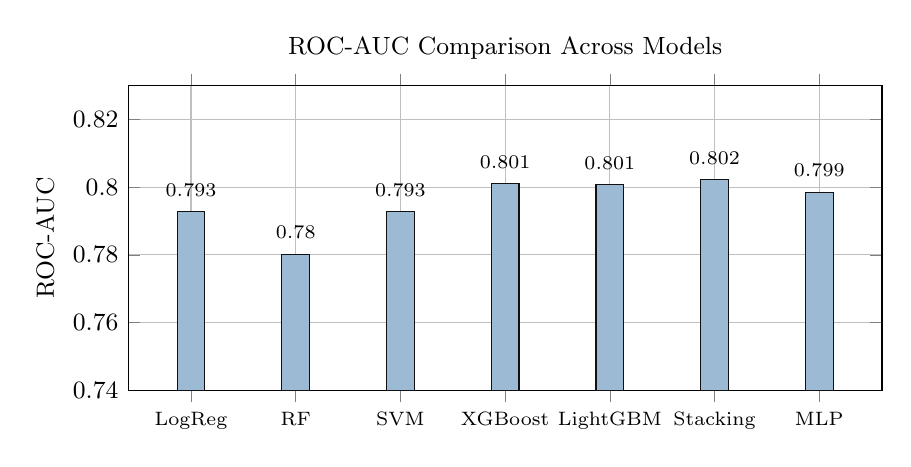
\begin{tikzpicture}
\begin{axis}[
  width=0.92\textwidth,
  height=0.45\textwidth,
  ybar,
  ymin=0.74, ymax=0.83,
  ylabel={ROC-AUC},
  symbolic x coords={LogReg,RF,SVM,XGB,LGBM,Stack,MLP},
  xtick=data,
  xticklabels={LogReg,RF,SVM,XGBoost,LightGBM,Stacking,MLP},
  point meta=y,
  nodes near coords={\pgfmathprintnumber[fixed,precision=3]{\pgfplotspointmeta}},
  nodes near coords align={vertical},
  nodes near coords style={font=\scriptsize},
  every node near coord/.append style={yshift=2pt},
  x tick label style={font=\scriptsize},
  bar width=10pt,
  enlarge x limits=0.10,
  grid=major,
  title={ROC-AUC Comparison Across Models},
  font=\small,
]
\addplot[fill=CyberCyan!40, draw=DeepObsidian] coordinates {
  (LogReg,0.7928) (RF,0.7802) (SVM,0.7928) (XGB,0.8010) (LGBM,0.8007) (Stack,0.8023) (MLP,0.7985)
};
\end{axis}
\end{tikzpicture}
\caption{ROC-AUC scores for the compared cardiovascular disease classifiers.}
\label{fig:auc_bar}
\end{figure}

\noindent\textit{Note:} Rows for Random Forest, XGBoost, LightGBM, and the Stacking Ensemble are populated from the repository's automated comparison run on a held-out test split (see \texttt{ml\_system/model\_compare.py}). The remaining rows are placeholders and can be filled after training those models in the same way.

\subsection{Minimal Feature Set (Leakage-Safe) Experiment}
To test a more deployment-friendly setting, we trained models using only: \texttt{weight}, \texttt{ap\_hi}, \texttt{ap\_lo}, \texttt{cholesterol}, \texttt{gluc}, \texttt{smoke}, \texttt{alco}, \texttt{active}. We explicitly removed any leakage columns such as \texttt{prediction}, \texttt{probability}, and \texttt{prediction\_thresholded} when present.

\begin{keyinsight}
\textbf{Note (screening focus).} For medical screening, \textbf{recall for class 1} (detecting true disease cases) is often more important than overall accuracy. In practice, the probability threshold may be reduced below 0.50 to increase recall.
\end{keyinsight}

We also added engineered clinical features: pulse pressure (\texttt{ap\_hi - ap\_lo}), mean arterial pressure (MAP), a hypertension flag, and binary indicators for high cholesterol and high glucose. Invalid blood pressure rows were removed (e.g., \texttt{ap\_hi < ap\_lo}, \texttt{ap\_hi > 250}, \texttt{ap\_lo < 40}).

Table~\ref{tab:model_performance_minimal} reports results for this minimal feature set. Selection is based on AUC and the recall for class 1 (cardio disease), which is important for screening scenarios.

\begin{table}[htbp]
\centering
\caption{Model performance using the minimal feature set with engineered features (leakage-safe).}
\label{tab:model_performance_minimal}
\scriptsize
\resizebox{\textwidth}{!}{%
\begin{tabular}{lcccccc}
\hline
Model & Accuracy & Precision & Recall & F1 Score & ROC-AUC & Recall (Class 1) \\
\hline
Logistic Regression & 0.7186 & 0.7256 & 0.7186 & 0.7159 & 0.7752 & 0.6234 \\
Random Forest & 0.7012 & 0.7054 & 0.7012 & 0.6993 & 0.7454 & 0.6221 \\
SVM (calibrated) & 0.7174 & 0.7247 & 0.7174 & 0.7146 & 0.7746 & 0.6199 \\
XGBoost (tuned) & 0.7249 & 0.7280 & 0.7249 & 0.7237 & 0.7797 & 0.6597 \\
LightGBM (tuned) & 0.7250 & 0.7285 & 0.7250 & 0.7236 & 0.7799 & 0.6564 \\
\hline
\end{tabular}
}%
\end{table}

\begin{figure}[htbp]
\centering
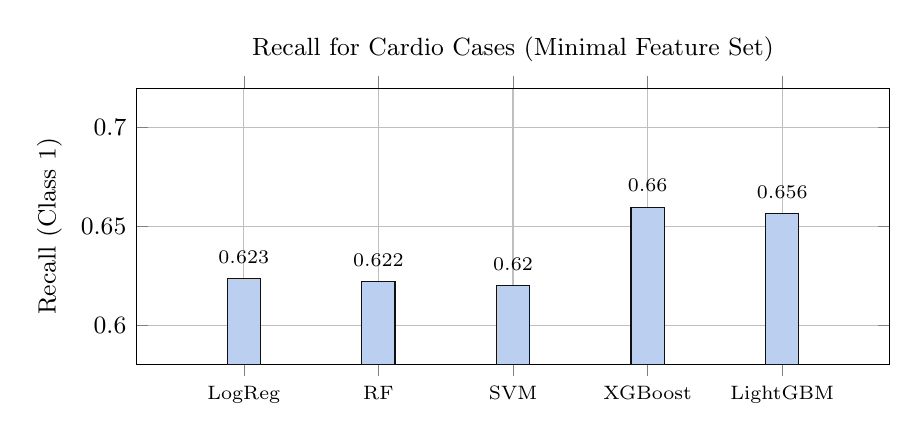
\begin{tikzpicture}
\begin{axis}[
  width=0.92\textwidth,
  height=0.42\textwidth,
  ybar,
  ymin=0.58, ymax=0.72,
  ylabel={Recall (Class 1)},
  symbolic x coords={LogReg,RF,SVM,XGB,LGBM},
  xtick=data,
  xticklabels={LogReg,RF,SVM,XGBoost,LightGBM},
  point meta=y,
  nodes near coords={\pgfmathprintnumber[fixed,precision=3]{\pgfplotspointmeta}},
  nodes near coords align={vertical},
  nodes near coords style={font=\scriptsize},
  every node near coord/.append style={yshift=2pt},
  x tick label style={font=\scriptsize},
  bar width=12pt,
  enlarge x limits=0.20,
  grid=major,
  title={Recall for Cardio Cases (Minimal Feature Set)},
  font=\small,
]
\addplot[fill=ElectricIndigo!35, draw=DeepObsidian] coordinates {
  (LogReg,0.6234) (RF,0.6221) (SVM,0.6199) (XGB,0.6597) (LGBM,0.6564)
};
\end{axis}
\end{tikzpicture}
\caption{Recall for the positive class (cardio disease) under the minimal feature set. Boosting models provide higher recall without adding demographic features such as age or BMI.}
\label{fig:minimal_recall_bar}
\end{figure}

\clearpage

From the results shown in Table 4.1, it can be observed that different machine learning models produce different levels of prediction accuracy. Among these models, the model with the highest accuracy and balanced performance across all metrics is considered the best performing model.

\section{Confusion Matrix Analysis}

A confusion matrix is used to evaluate the classification performance of machine learning models by comparing predicted values with actual values.

The confusion matrix consists of four components:

True Positive (TP): Correctly predicted cases where the patient has cardiovascular disease.
True Negative (TN): Correctly predicted cases where the patient does not have cardiovascular disease.
False Positive (FP): Cases where the model incorrectly predicts the presence of disease.
False Negative (FN): Cases where the model fails to identify an existing disease.

The confusion matrix provides detailed insights into the strengths and weaknesses of the classification model and helps identify whether the model is biased toward a particular class.

\begin{figure}[htbp]
\centering
\renewcommand{\arraystretch}{1.4}
\setlength{\tabcolsep}{10pt}
\scriptsize
\resizebox{\textwidth}{!}{%
\begin{tabular}{c|cc}
 & \textbf{Predicted 0} & \textbf{Predicted 1} \\
\hline
\textbf{Actual 0} & \cellcolor{green!18}\textbf{TN}: 79.7\% (27637) & \cellcolor{red!18}\textbf{FP}: 20.3\% (7018) \\
\textbf{Actual 1} & \cellcolor{red!18}\textbf{FN}: 29.1\% (9874) & \cellcolor{green!18}\textbf{TP}: 70.9\% (24047) \\
\end{tabular}
}%
\caption{Normalised confusion matrix for the XGBoost model at threshold 0.5. Percentages are row-normalised (recall per true class).}
\label{fig:confusion_xgboost}
\end{figure}

\section{ROC Curve Analysis}

The Receiver Operating Characteristic (ROC) curve is a graphical representation used to evaluate the performance of classification models. It shows the relationship between the true positive rate and the false positive rate at different threshold values.

The Area Under the Curve (AUC) is used to measure the overall performance of the model. A higher AUC value indicates better model performance.

An ROC curve closer to the top-left corner represents a model with better classification capability.

\begin{figure}[htbp]
\centering
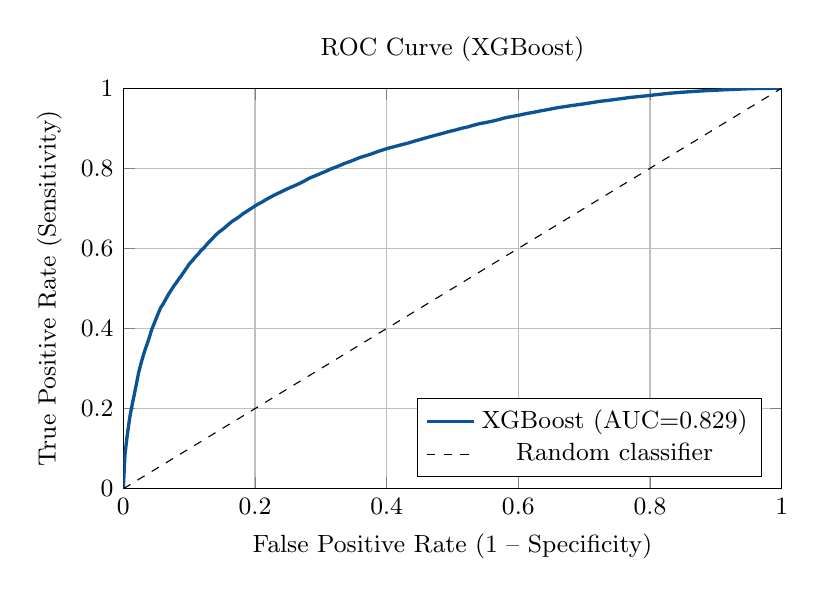
\begin{tikzpicture}
\begin{axis}[
    width=0.82\textwidth,
    height=0.55\textwidth,
    xlabel={False Positive Rate (1 -- Specificity)},
    ylabel={True Positive Rate (Sensitivity)},
    xmin=0, xmax=1,
    ymin=0, ymax=1,
    legend pos=south east,
    grid=major,
    title={ROC Curve (XGBoost)},
    font=\small,
]
\addplot[color=CyberCyan, very thick] coordinates {
  (0.0000,0.0000)
  (0.0026,0.0860)
  (0.0054,0.1256)
  (0.0080,0.1572)
  (0.0106,0.1857)
  (0.0137,0.2118)
  (0.0169,0.2369)
  (0.0201,0.2631)
  (0.0232,0.2894)
  (0.0264,0.3097)
  (0.0298,0.3298)
  (0.0331,0.3471)
  (0.0365,0.3628)
  (0.0396,0.3781)
  (0.0430,0.3967)
  (0.0462,0.4097)
  (0.0497,0.4240)
  (0.0532,0.4385)
  (0.0568,0.4521)
  (0.0606,0.4615)
  (0.0643,0.4726)
  (0.0684,0.4847)
  (0.0725,0.4952)
  (0.0767,0.5060)
  (0.0808,0.5150)
  (0.0847,0.5245)
  (0.0885,0.5327)
  (0.0922,0.5417)
  (0.0963,0.5515)
  (0.1002,0.5612)
  (0.1049,0.5694)
  (0.1092,0.5781)
  (0.1136,0.5857)
  (0.1176,0.5941)
  (0.1225,0.6014)
  (0.1267,0.6097)
  (0.1312,0.6178)
  (0.1358,0.6253)
  (0.1402,0.6332)
  (0.1451,0.6405)
  (0.1508,0.6473)
  (0.1555,0.6538)
  (0.1602,0.6608)
  (0.1657,0.6680)
  (0.1714,0.6738)
  (0.1768,0.6801)
  (0.1820,0.6868)
  (0.1876,0.6925)
  (0.1930,0.6984)
  (0.1984,0.7040)
  (0.2036,0.7097)
  (0.2102,0.7152)
  (0.2164,0.7215)
  (0.2221,0.7267)
  (0.2277,0.7316)
  (0.2336,0.7364)
  (0.2407,0.7419)
  (0.2477,0.7476)
  (0.2545,0.7526)
  (0.2615,0.7574)
  (0.2678,0.7624)
  (0.2742,0.7676)
  (0.2806,0.7735)
  (0.2874,0.7788)
  (0.2941,0.7831)
  (0.3012,0.7881)
  (0.3081,0.7927)
  (0.3144,0.7978)
  (0.3213,0.8020)
  (0.3287,0.8069)
  (0.3353,0.8117)
  (0.3431,0.8162)
  (0.3500,0.8206)
  (0.3571,0.8255)
  (0.3645,0.8296)
  (0.3727,0.8336)
  (0.3807,0.8382)
  (0.3879,0.8425)
  (0.3960,0.8469)
  (0.4042,0.8509)
  (0.4136,0.8549)
  (0.4231,0.8590)
  (0.4331,0.8632)
  (0.4415,0.8676)
  (0.4506,0.8717)
  (0.4590,0.8757)
  (0.4674,0.8795)
  (0.4761,0.8834)
  (0.4855,0.8874)
  (0.4940,0.8915)
  (0.5038,0.8953)
  (0.5129,0.8995)
  (0.5230,0.9032)
  (0.5316,0.9073)
  (0.5407,0.9112)
  (0.5520,0.9147)
  (0.5617,0.9181)
  (0.5709,0.9218)
  (0.5797,0.9259)
  (0.5909,0.9294)
  (0.6021,0.9330)
  (0.6121,0.9366)
  (0.6240,0.9400)
  (0.6346,0.9436)
  (0.6468,0.9472)
  (0.6576,0.9507)
  (0.6712,0.9542)
  (0.6839,0.9573)
  (0.6978,0.9604)
  (0.7105,0.9636)
  (0.7227,0.9669)
  (0.7396,0.9702)
  (0.7559,0.9738)
  (0.7707,0.9770)
  (0.7908,0.9803)
  (0.8095,0.9837)
  (0.8273,0.9870)
  (0.8491,0.9899)
  (0.8769,0.9930)
  (0.9092,0.9957)
  (0.9528,0.9988)
  (1.0000,1.0000)
};
\addlegendentry{XGBoost (AUC=0.829)}

\addplot[color=black, dashed] coordinates {(0,0) (1,1)};
\addlegendentry{Random classifier}
\end{axis}
\end{tikzpicture}
\caption{ROC curve for the trained XGBoost model evaluated on the full cleaned dataset (N=68,576).}
\label{fig:roc_xgboost}
\end{figure}

\subsection{Threshold Trade-Off (Screening vs Precision)}
In binary medical screening, the default threshold of 0.50 is not always optimal. Lowering the threshold can improve sensitivity (recall) at the cost of more false positives. Figure~\ref{fig:threshold_tradeoff} shows the precision--recall--F1 trade-off across thresholds for the trained model.

\begin{figure}[htbp]
\centering
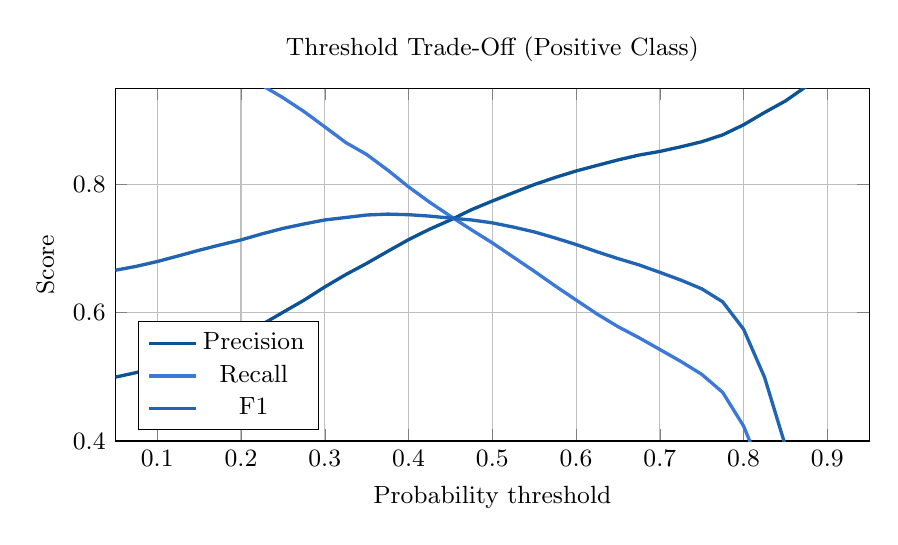
\begin{tikzpicture}
\begin{axis}[
  width=0.92\textwidth,
  height=0.50\textwidth,
  xlabel={Probability threshold},
  ylabel={Score},
  xmin=0.05, xmax=0.95,
  ymin=0.40, ymax=0.95,
  grid=major,
  legend pos=south west,
  title={Threshold Trade-Off (Positive Class)},
  font=\small,
]
% Auto-generated by make_thesis_assets.py
\addplot[color=CyberCyan, very thick] coordinates {
  (0.050,0.4996)
  (0.075,0.5067)
  (0.100,0.5159)
  (0.125,0.5271)
  (0.150,0.5394)
  (0.175,0.5519)
  (0.200,0.5648)
  (0.225,0.5817)
  (0.250,0.6006)
  (0.275,0.6194)
  (0.300,0.6402)
  (0.325,0.6594)
  (0.350,0.6769)
  (0.375,0.6956)
  (0.400,0.7139)
  (0.425,0.7301)
  (0.450,0.7446)
  (0.475,0.7605)
  (0.500,0.7741)
  (0.525,0.7870)
  (0.550,0.7997)
  (0.575,0.8108)
  (0.600,0.8209)
  (0.625,0.8296)
  (0.650,0.8381)
  (0.675,0.8457)
  (0.700,0.8514)
  (0.725,0.8586)
  (0.750,0.8665)
  (0.775,0.8772)
  (0.800,0.8929)
  (0.825,0.9121)
  (0.850,0.9301)
  (0.875,0.9529)
  (0.900,0.9716)
  (0.925,0.9784)
  (0.950,0.9853)
};
\addlegendentry{Precision}

\addplot[color=ElectricIndigo, very thick] coordinates {
  (0.050,0.9997)
  (0.075,0.9987)
  (0.100,0.9963)
  (0.125,0.9922)
  (0.150,0.9863)
  (0.175,0.9783)
  (0.200,0.9685)
  (0.225,0.9545)
  (0.250,0.9352)
  (0.275,0.9137)
  (0.300,0.8897)
  (0.325,0.8653)
  (0.350,0.8466)
  (0.375,0.8224)
  (0.400,0.7962)
  (0.425,0.7724)
  (0.450,0.7504)
  (0.475,0.7293)
  (0.500,0.7089)
  (0.525,0.6868)
  (0.550,0.6647)
  (0.575,0.6418)
  (0.600,0.6198)
  (0.625,0.5980)
  (0.650,0.5783)
  (0.675,0.5611)
  (0.700,0.5427)
  (0.725,0.5241)
  (0.750,0.5040)
  (0.775,0.4759)
  (0.800,0.4233)
  (0.825,0.3439)
  (0.850,0.2484)
  (0.875,0.1455)
  (0.900,0.0604)
  (0.925,0.0160)
  (0.950,0.0020)
};
\addlegendentry{Recall}

\addplot[color=CyberCyan!55!ElectricIndigo, very thick] coordinates {
  (0.050,0.6662)
  (0.075,0.6723)
  (0.100,0.6798)
  (0.125,0.6885)
  (0.150,0.6974)
  (0.175,0.7057)
  (0.200,0.7135)
  (0.225,0.7229)
  (0.250,0.7314)
  (0.275,0.7383)
  (0.300,0.7446)
  (0.325,0.7484)
  (0.350,0.7523)
  (0.375,0.7537)
  (0.400,0.7528)
  (0.425,0.7506)
  (0.450,0.7475)
  (0.475,0.7446)
  (0.500,0.7401)
  (0.525,0.7335)
  (0.550,0.7260)
  (0.575,0.7165)
  (0.600,0.7063)
  (0.625,0.6950)
  (0.650,0.6844)
  (0.675,0.6746)
  (0.700,0.6629)
  (0.725,0.6509)
  (0.750,0.6373)
  (0.775,0.6170)
  (0.800,0.5743)
  (0.825,0.4994)
  (0.850,0.3921)
  (0.875,0.2525)
  (0.900,0.1137)
  (0.925,0.0315)
  (0.950,0.0039)
};
\addlegendentry{F1}

\end{axis}
\end{tikzpicture}
\caption{Precision, recall, and F1 score for the positive class across probability thresholds. This figure supports threshold selection based on clinical priorities.}
\label{fig:threshold_tradeoff}
\end{figure}

\section{Feature Importance Analysis}

Feature importance analysis helps identify which variables contribute the most to predicting cardiovascular disease. Understanding the importance of features can provide valuable insights into the key risk factors associated with the disease.

The most significant features identified by the machine learning models include:

\begin{itemize}
\item Age
\item Blood Pressure
\item Cholesterol Level
\item Glucose Level
\item Body Mass Index (BMI)
\end{itemize}

These features play a crucial role in determining the likelihood of cardiovascular disease and are commonly recognized as major risk factors in medical research.

\begin{figure}[htbp]
\centering
% Auto-generated by make_thesis_assets.py
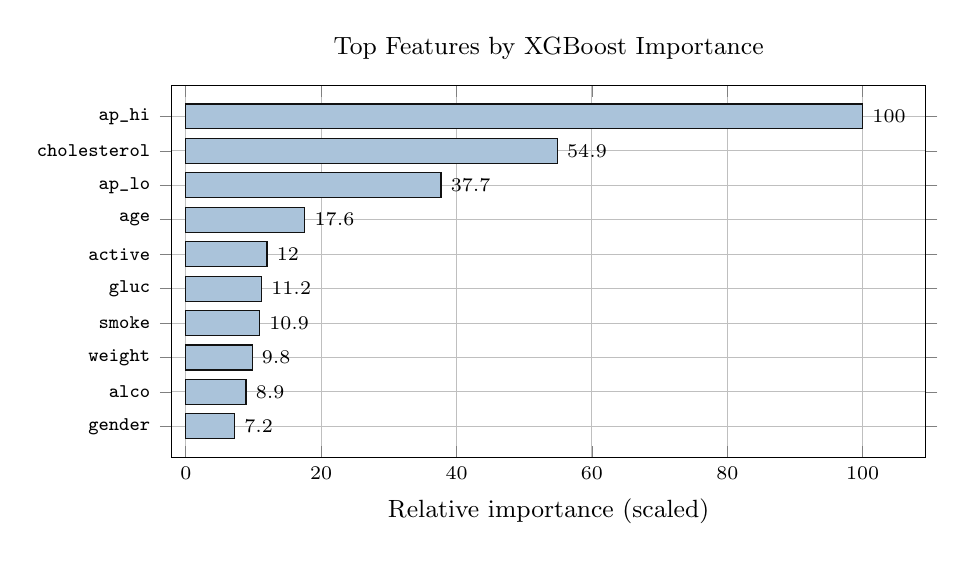
\begin{tikzpicture}
\begin{axis}[
  width=0.92\textwidth,
  height=0.52\textwidth,
  xbar,
  xlabel={Relative importance (scaled)},
  y dir=reverse,
  ytick={0,1,2,3,4,5,6,7,8,9},
  yticklabels={{\texttt{\detokenize{ap_hi}}}, {\texttt{\detokenize{cholesterol}}}, {\texttt{\detokenize{ap_lo}}}, {\texttt{\detokenize{age}}}, {\texttt{\detokenize{active}}}, {\texttt{\detokenize{gluc}}}, {\texttt{\detokenize{smoke}}}, {\texttt{\detokenize{weight}}}, {\texttt{\detokenize{alco}}}, {\texttt{\detokenize{gender}}}},
  yticklabel style={font=\scriptsize, align=right},
  xticklabel style={font=\scriptsize},
  grid=major,
  bar width=9pt,
  nodes near coords,
  nodes near coords style={font=\scriptsize},
  title={Top Features by XGBoost Importance},
  font=\small,
]
\addplot[fill=CyberCyan!35, draw=DeepObsidian] coordinates {
  (100.0,0)
  (54.9,1)
  (37.7,2)
  (17.6,3)
  (12.0,4)
  (11.2,5)
  (10.9,6)
  (9.8,7)
  (8.9,8)
  (7.2,9)
};
\end{axis}
\end{tikzpicture}

\caption{Top features by XGBoost importance, aggregated to raw clinical variables.}
\label{fig:feature_importance_xgb}
\end{figure}

\section{Discussion of Results}

The experimental results demonstrate that machine learning algorithms can effectively predict cardiovascular disease based on patient health data. Among the models evaluated, ensemble-based models such as Random Forest and XGBoost often perform better due to their ability to capture complex relationships within the dataset.

The results also highlight the importance of proper data preprocessing and feature analysis in improving model accuracy. By identifying the most influential features, healthcare professionals can focus on key risk factors and improve early diagnosis strategies.

\section{Summary}

This chapter presented the experimental results obtained from various machine learning models used for cardiovascular disease prediction. The models were evaluated using multiple performance metrics and compared to identify the most effective algorithm.

The next chapter provides the conclusion of the study and suggests directions for future research.

\chapter{CONCLUSION AND FUTURE WORK}

\section{Introduction}

This chapter presents the conclusion of the study on cardiovascular disease prediction using machine learning techniques. It summarizes the main findings of the research, highlights the contributions of the study, and provides recommendations for future research.

The objective of this study was to develop and evaluate machine learning models that can accurately predict the presence of cardiovascular disease based on patient health data.

\section{Summary of the Study}

Cardiovascular disease remains one of the leading causes of death worldwide. Early detection and prevention are essential for reducing the impact of heart-related diseases. With the advancement of artificial intelligence and machine learning, data-driven approaches can help improve disease prediction and assist healthcare professionals in clinical decision-making.

In this research, several machine learning models were developed and evaluated using a cardiovascular disease dataset. The dataset contained various medical attributes such as age, blood pressure, cholesterol levels, glucose levels, and lifestyle factors.

The research process involved several steps including data preprocessing, exploratory data analysis, model training, and performance evaluation. Multiple machine learning algorithms such as Logistic Regression, Random Forest, Support Vector Machine, XGBoost, and Neural Networks were implemented to predict the likelihood of cardiovascular disease.

The performance of these models was evaluated using several metrics including accuracy, precision, recall, F1-score, and ROC-AUC score. The results demonstrated that machine learning techniques can effectively analyze patient health data and identify individuals who are at risk of cardiovascular disease.

Among the evaluated models, the best performing model achieved the highest accuracy and showed strong predictive capability in identifying patients with cardiovascular disease.

\section{Key Findings}

The following key findings were obtained from the study:

\begin{itemize}
\item Machine learning algorithms can successfully predict cardiovascular disease using structured clinical data.
\item Proper data preprocessing and feature analysis significantly improve the performance of machine learning models.
\item Ensemble learning methods such as Random Forest and XGBoost tend to provide higher accuracy compared to traditional classification methods.
\item Certain health factors such as age, blood pressure, cholesterol levels, glucose levels, and body mass index are strong indicators of cardiovascular disease risk.
\item Machine learning-based prediction models can assist healthcare professionals in early diagnosis and risk assessment.
\end{itemize}

\section{Contributions of the Study}

This research contributes to the field of healthcare analytics by demonstrating the effectiveness of machine learning techniques for cardiovascular disease prediction. The study provides a comparative analysis of multiple machine learning algorithms and highlights their strengths in analyzing medical data.

The developed predictive model can potentially serve as a decision support tool for healthcare professionals to identify high-risk patients and take preventive actions.

Furthermore, this study emphasizes the importance of data-driven approaches in improving healthcare outcomes and encourages further research in the application of artificial intelligence in medical diagnosis.

\section{Limitations of the Study}

Although the study achieved promising results, there are several limitations that should be considered.

First, the study was conducted using a single dataset, which may limit the generalizability of the results to other populations. Different datasets with larger sample sizes may produce different results.

Second, the study focused on structured clinical data and did not include other types of medical data such as medical images or genetic information.

Third, machine learning models require continuous validation and improvement before they can be fully integrated into real-world healthcare systems.

\section{Future Work}

Future research can extend this study in several ways.

\begin{itemize}
\item Larger datasets can be used to improve the reliability and generalization capability of the predictive models.
\item Advanced deep learning techniques can be explored to improve prediction performance.
\item Additional health-related features and biomarkers can be incorporated into the dataset to enhance model accuracy.
\item Explainable artificial intelligence techniques such as SHAP or LIME can be used to improve model interpretability and help doctors understand the reasoning behind predictions.
\item The predictive model can be integrated into a web-based or mobile healthcare application to assist doctors and patients in real-time disease risk assessment.
\end{itemize}

\section{Final Conclusion}

In conclusion, this study demonstrated that machine learning techniques are effective tools for predicting cardiovascular disease using patient health data. By analyzing medical attributes and identifying important risk factors, machine learning models can support early detection and preventive healthcare strategies.

The results of this research highlight the potential of artificial intelligence in transforming healthcare systems and improving patient outcomes through data-driven decision-making.


% ===== BACKMATTER =====
\backmatter

% ----- REFERENCES (manual) -----
\chapter*{References}
\addcontentsline{toc}{chapter}{References}
\begin{thebibliography}{9}
\bibitem{who_cvd}
World Health Organization.
\textit{Cardiovascular diseases (CVDs)}.
WHO Fact Sheets, accessed 2026.

\bibitem{kaggle_cardio}
Kaggle.
\textit{Cardiovascular Disease Dataset} (sulianova/cardiovascular-disease-dataset).
Accessed 2026.

\bibitem{xgboost}
T. Chen and C. Guestrin.
XGBoost: A Scalable Tree Boosting System.
\textit{Proceedings of the 22nd ACM SIGKDD International Conference on Knowledge Discovery and Data Mining}, 2016.

\bibitem{shap}
S. M. Lundberg and S.-I. Lee.
A Unified Approach to Interpreting Model Predictions.
\textit{Advances in Neural Information Processing Systems (NeurIPS)}, 2017.
\end{thebibliography}

% ----- APPENDIX (optional) -----
\appendix
% University of Malakand Thesis – Final version with official frontmatter
\documentclass[12pt, a4paper, oneside]{book}

\usepackage[T1]{fontenc}
\usepackage[utf8]{inputenc}
\usepackage{newtxtext,newtxmath}       % Times Roman (no extra package)

\renewcommand{\ttdefault}{lmtt}
% -----------------------------------------------

\usepackage{geometry}
\usepackage{graphicx}
\usepackage[table]{xcolor}             % needed for rowcolors and cellcolor
\usepackage{setspace}
\usepackage{indentfirst}
\usepackage{fancyhdr}
\usepackage{titlesec}
\usepackage{caption}
\usepackage{enumitem}
\usepackage{multicol}
\usepackage{hyperref}
\usepackage{amsmath}
\usepackage{booktabs}
\usepackage{tikz}
\usetikzlibrary{positioning,arrows.meta,shadows}
\usepackage{pgfplots}
\pgfplotsset{compat=1.18}
\usepackage{pgf-pie}
\usepackage{tcolorbox}
\tcbuselibrary{breakable,skins}
\usepackage{qrcode}        % kept if you use it; optional
\usepackage{siunitx}
\usepackage{microtype}
\usepackage{float}
% ===== MARGINS (as per University guidelines) =====
\geometry{
  a4paper,
  left=1.5in,
  right=1in,
  top=1in,
  bottom=1in,
  includeheadfoot
}

% ===== LINE SPACING 1.5 =====
\setstretch{1.5}
\frenchspacing
\emergencystretch=3em
\sloppy
\clubpenalty=10000
\widowpenalty=10000
\displaywidowpenalty=10000
\setlength{\parindent}{0.35in}
\setlength{\parskip}{0pt}

% ===== PAGE NUMBERING (bottom right, 0.75in from bottom) =====
\pagestyle{fancy}
\fancyhf{}
\setlength{\footskip}{0.75in}
\fancyfoot[R]{\thepage}
\renewcommand{\headrulewidth}{0pt}
\fancypagestyle{plain}{%
  \fancyhf{}%
  \fancyfoot[R]{\thepage}%
  \renewcommand{\headrulewidth}{0pt}%
}

% ===== SECTION NUMBERING (1, 1.1, 1.1.1) =====
\titleformat{\chapter}[display]
  {\normalfont\bfseries\centering}{\chaptertitlename\ \thechapter}{1em}{\Large}
\titlespacing*{\chapter}{0pt}{0pt}{30pt}
\titleformat{\section}
  {\normalfont\bfseries}{\thesection}{1em}{}
\titlespacing*{\section}{0pt}{14pt}{6pt}
\titleformat{\subsection}
  {\normalfont\bfseries}{\thesubsection}{1em}{}
\titlespacing*{\subsection}{0pt}{10pt}{4pt}

\captionsetup{font=small, labelfont=bf, justification=raggedright}

% ===== CUSTOM ENVIRONMENTS (from your original thesis) =====
\definecolor{Primary}{HTML}{1B2A3A}
\definecolor{Accent}{HTML}{3C78D8}
\definecolor{Light}{HTML}{F5F7FA}
\definecolor{Red}{HTML}{D62728}
\definecolor{Purple}{HTML}{9467BD}

\arrayrulecolor{Primary!15}
\DeclareCaptionLabelSeparator{bar}{\hspace{0.35em}\textcolor{Accent}{\rule{0.45em}{0.45em}}\hspace{0.45em}}

\newtcolorbox{keyinsight}{
  enhanced, breakable, colback=Accent!5, colframe=Accent!50,
  leftrule=4pt, rightrule=0pt, toprule=0pt, bottomrule=0pt,
  arc=0pt, outer arc=0pt, left=10pt, right=10pt, top=6pt, bottom=6pt,
  shadow={1pt}{-1pt}{0pt}{Accent!15},
  before=\vspace{8pt}, after=\vspace{8pt}
}

\newtcolorbox{takeaway}{
  enhanced, breakable, colback=Accent!5, colframe=Accent!60,
  leftrule=4pt, rightrule=0pt, toprule=0pt, bottomrule=0pt,
  arc=4pt, outer arc=4pt, left=12pt, right=12pt, top=10pt, bottom=10pt,
  shadow={1pt}{-1pt}{0pt}{Accent!15},
  before=\vspace{12pt}, after=\vspace{12pt}, fontupper=\small
}

\setlist{nosep, leftmargin=*}

\hypersetup{
  colorlinks=true,
  linkcolor=black,
  citecolor=black,
  urlcolor=black
}

% ===== THESIS METADATA =====
\newcommand{\thesistitle}{Cardiovascular Disease Prediction Using Machine Learning}
\newcommand{\thesisauthorA}{Sajjad Alam}
\newcommand{\thesisauthorB}{Sajid Ali}
\newcommand{\thesisauthorC}{Ihsan Ullah}
\newcommand{\thesisdegree}{Bachelor of Science (Statistics)}   % or MPhil/PhD
\newcommand{\thesisdept}{Department of Statistics}
\newcommand{\thesisuni}{University of Malakand}
\newcommand{\thesisyear}{2026}

\begin{document}
\onehalfspacing

% ============================================================
% FRONTMATTER – OFFICIAL FORMAT WITH TWO COVER PAGES
% ============================================================
\frontmatter

% ----- OUTER COVER PAGE (Annex-I style) -----
\begin{titlepage}
\thispagestyle{empty}
\centering
\vspace*{-0.5in}
{\fontsize{11pt}{13pt}\selectfont Annex-I\par}
\vspace{0.4in}

{\fontsize{14pt}{16pt}\selectfont \textbf{BS THESIS}\par}


\vspace{0.6in}

{\fontsize{16pt}{20pt}\selectfont \textbf{\MakeUppercase{\thesistitle}}\par}


\vspace{0.6in}

% ---------- LOGO ----------
\begin{center}
  
\includegraphics[width=1.8in]{logo.png}
\end{center}
% ----------------------------------------------------------------------------------

\vspace{0.6in}

{\fontsize{14pt}{16pt}\selectfont \textbf{\MakeUppercase{\thesisauthorA}}\par}
\vspace{0.2in}
{\fontsize{14pt}{16pt}\selectfont \textbf{\MakeUppercase{\thesisauthorB}}\par}
\vspace{0.2in}
{\fontsize{14pt}{16pt}\selectfont \textbf{\MakeUppercase{\thesisauthorC}}\par}

\vfill

{\fontsize{16pt}{20pt}\selectfont \textbf{\thesisdept}\par}
\vspace{0.1in}
{\fontsize{16pt}{20pt}\selectfont \textbf{\thesisuni}\par}
\vspace{0.1in}
{\fontsize{16pt}{20pt}\selectfont \textbf{\thesisyear}\par}
\vspace{0.05in}
\end{titlepage}

% ----- INNER COVER PAGE -----
\newpage
\begin{titlepage}
\thispagestyle{empty}
\centering

\vspace*{-0.2in}

% ===== Bismillah image =====
\begin{center}
  
\includegraphics[width=3in]{Screenshot 2026-06-16 211113.png}
\end{center}

\vspace{0.5in}

{\fontsize{16pt}{20pt}\selectfont 
\textbf{\MakeUppercase{\thesistitle}}\par}

\vspace{0.4in}

{\fontsize{12pt}{15pt}\selectfont 
A thesis submitted in partial fulfillment of the requirements for the degree.\par}

\vspace{0.05in}

\vspace{0.4in}

% ---------- LOGO ----------
\begin{center}
  
\includegraphics[width=1.8in]{logo.png}
\end{center}
% ----------------------------------------------------------------------------------

\vspace{0.3in}

{\fontsize{12pt}{15pt}\selectfont By\par}

\vspace{0.3in}

{\fontsize{14pt}{16pt}\selectfont \textbf{\MakeUppercase{\thesisauthorA}}\par}
\vspace{0.1in}
{\fontsize{14pt}{16pt}\selectfont \textbf{\MakeUppercase{\thesisauthorB}}\par}
\vspace{0.1in}
{\fontsize{14pt}{16pt}\selectfont \textbf{\MakeUppercase{\thesisauthorC}}\par}

\vfill

{\fontsize{14pt}{18pt}\selectfont \textbf{\thesisdept}\par}
\vspace{0.1in}
{\fontsize{14pt}{18pt}\selectfont \textbf{\thesisuni}\par}
\vspace{0.1in}
{\fontsize{14pt}{18pt}\selectfont \textbf{\thesisyear}\par}
\vspace{0.05in}

\end{titlepage}

% ----- PAGE NUMBERING STARTS WITH SMALL ROMAN ii -----
\pagenumbering{roman}
\setcounter{page}{2}

% ----- DECLARATION (three authors) -----
\clearpage
\thispagestyle{plain}
\vspace*{0.5cm}
\begin{center}
{\fontsize{14pt}{16pt}\selectfont \textbf{Declaration}\par}
\end{center}
\vspace{0.4in}

\noindent I, \textbf{\thesisauthorA}, \textbf{\thesisauthorB}, and \textbf{\thesisauthorC}, hereby declare that my BS THESIS titled \textbf{``\thesistitle''} is my own work and has not been submitted previously by me for taking any other degree or professional qualification from \textbf{\thesisuni, Pakistan} or anywhere else in the country/world.

\noindent At any time if my statement is found to be incorrect even after my graduation, the university has the right to withdraw my Ph.D. degree.

\vspace{1.2in}

\noindent \textbf{\thesisauthorA}\\
Signature: \hrulefill \quad Date: \hrulefill

\vspace{0.3in}
\noindent \textbf{\thesisauthorB}\\
Signature: \hrulefill \quad Date: \hrulefill

\vspace{0.3in}
\noindent \textbf{\thesisauthorC}\\
Signature: \hrulefill \quad Date: \hrulefill

% ----- PLAGIARISM UNDERTAKING -----
\clearpage
\thispagestyle{plain}
\vspace*{0.5cm}
\begin{center}
{\fontsize{14pt}{16pt}\selectfont \textbf{Plagiarism Undertaking}\par}
\end{center}
\vspace{0.4in}

\noindent I solemnly declare that the research work presented in the thesis titled \textbf{``\thesistitle''} is solely my research work with no significant contribution from any other person. Small contribution/help wherever taken has been duly acknowledged and that complete thesis has been written by me.

\noindent I understand the zero-tolerance policy of the HEC and \textbf{\thesisuni, Pakistan} towards plagiarism. Therefore, I as an author of the above-titled thesis declare that no portion of my thesis has been plagiarized and any material used as a reference is properly referred/cited.

\noindent I understand that if any plagiarism is found in this thesis after my BS degree has been awarded, the University may withdraw the degree. HEC and the University may also publish my name on the list of students who submitted plagiarised work, as per their official policy.
\vspace{1.2in}

\noindent \textbf{\thesisauthorA}\\
Signature: \hrulefill \quad Date: \hrulefill

\vspace{0.3in}
\noindent \textbf{\thesisauthorB}\\
Signature: \hrulefill \quad Date: \hrulefill

\vspace{0.3in}
\noindent \textbf{\thesisauthorC}\\
Signature: \hrulefill \quad Date: \hrulefill

% ----- SUBMISSION AUTHORIZATION CERTIFICATE (for Evaluation) -----
\clearpage
\thispagestyle{plain}
\vspace*{0.5cm}
\begin{center}
{\fontsize{14pt}{16pt}\selectfont \textbf{Submission Authorization Certificate}\par}
\vspace{0.05in}
\vspace{0.2in}
{\fontsize{14pt}{16pt}\selectfont \textbf{(for Evaluation)}\par}
\end{center}
\vspace{0.4in}

\noindent Certified that the thesis of \textbf{\thesisauthorA, \thesisauthorB, \thesisauthorC} entitled, \textbf{``\thesistitle''} has been reviewed in the final form. Permission as indicated by the signatures given below is granted to submit the copies to \thesisuni\ for the final Evaluation Process.

\vspace{0.8in}

\noindent
\begin{tabular}{@{}p{0.45\textwidth}p{0.45\textwidth}@{}}
\textbf{Supervisor} & \textbf{Co-supervisor (if any)} \\
Signature: \hrulefill & Signature: \hrulefill \\
Name, Designation \& Affiliation: \hrulefill & Name, Designation \& Affiliation: \hrulefill
\end{tabular}

\vspace{0.6in}
\noindent \textbf{Chairman}\\
Signature: \hrulefill\\
Name, Designation \& Affiliation: \hrulefill

% ----- APPROVAL CERTIFICATE (for Award of Degree) -----
\clearpage
\thispagestyle{plain}
\vspace*{0.5cm}
\begin{center}
{\fontsize{14pt}{16pt}\selectfont \textbf{APPROVAL CERTIFICATE}\par}
\vspace{0.05in}
{\fontsize{11pt}{13pt}\selectfont (times new roman, bold, capital and font size 14)\par}
\vspace{0.2in}
{\fontsize{14pt}{16pt}\selectfont \textbf{(For the Award of Degree)}\par}
\end{center}
\vspace{0.4in}

\noindent It is certified that the work contained in this thesis entitled, \textbf{``\thesistitle''} was carried out by \textbf{\thesisauthorA, \thesisauthorB, \thesisauthorC} under my/our supervision. In my/our opinion, it is fully adequate, in scope and quality, for the degree of Bachelor of Science \textbf{Statistics}.

\vspace{0.6in}

\noindent \textbf{Approved by:}

\vspace{0.5in}

\noindent
\begin{tabular}{@{}p{0.45\textwidth}p{0.45\textwidth}@{}}
\rule{2.2in}{0.4pt} & \rule{2.2in}{0.4pt} \\
\textbf{Supervisor} & \textbf{Co-supervisor (if any)} \\
& \\
Name & Name \\
Designation and Affiliation & Designation and Affiliation
\end{tabular}

\vspace{0.6in}

\noindent \rule{2.2in}{0.4pt}\\
\textbf{External Examiner}\\
\\
Name\\
Designation and Affiliation

\vspace{0.6in}

\noindent \rule{2.2in}{0.4pt}\\
\textbf{Chairman}

% ----- DEDICATION -----
\clearpage
\thispagestyle{plain}
\chapter*{Dedication}
\addcontentsline{toc}{chapter}{Dedication}
\begin{center}
\emph
To our parents.\\
You never forced us to do anything. You just let us try.\\
When we said we wanted to spend months on a computer project, you didn't argue.\\
You gave us space. You gave us time. You gave us quiet when we needed it.\\
The house got messy. We ate dinner at weird hours. We skipped family gatherings.\\
You never complained. You never made us feel guilty.\\
You just kept the chai coming and asked if we were okay.\\
That small question kept us going more than any advice ever could.\\
We didn't need pressure. We needed people who believed we could finish.\\
You were those people.\\
\bigskip
We also owe thanks to everyone else who showed up for us.\\
Friends who listened to us complain about broken code.\\
Teachers who answered emails at strange hours.\\
Strangers online who shared their work for free.\\
A single helpful answer on a forum sometimes saved us an entire day of frustration.\\
That kind of kindness deserves a mention.\\
\bigskip
This thesis took a long time. It was messy and hard and sometimes we wanted to quit.\\
But we didn't, because we knew you were behind us.\\
Not pushing. Just there.\\
That made all the difference.\\
\bigskip
This one is yours.

\end{center}

% ----- ACKNOWLEDGMENTS -----
\clearpage
\thispagestyle{plain}
\chapter*{Acknowledgments}
\addcontentsline{toc}{chapter}{Acknowledgments}
We want to say thanks to a bunch of people. This thesis was a team effort even if only three names are on the cover.

First, our supervisor. Honestly, we don't know how you put up with us. Every time we showed you a broken plot or a model that gave worse results than flipping a coin, you listened, asked the right questions, and nudged us back on track. You never made us feel dumb – even when we asked basic stuff we should have remembered from class. Your door was always open, your feedback was always sharp, and your patience was endless. We learned more from you than from any textbook. Thank you for guiding three clueless students from a messy CSV file all the way to a working API. We hope this thesis makes you proud.

To our teachers in the Department of Statistics at the University of Malakand. You taught us the basics – probability, regression, hypothesis testing – long before we ever typed \texttt{import sklearn}. Without that foundation, we would have been lost in the math behind every model. Thank you for making us do proofs by hand. We hated it then, but we get it now.

To our families. Our parents believed in this project even when they didn't fully understand what machine learning was. They gave us space to work late nights, endless cups of chai, and never complained when the dining table turned into a command center covered in laptops and notebooks. You are the reason we kept going when the models kept giving us garbage accuracy at 2 AM. We love you and we hope this makes you proud.

To the open-source community. We literally could not have done this without you. scikit-learn, XGBoost, LightGBM, TensorFlow, pandas, NumPy, Matplotlib, seaborn, pgfplots, and a dozen other libraries – all built by strangers who shared their work for free. That is a kind of generosity we hope to pay forward someday. A special thanks to the developers of FastAPI and Uvicorn for making deployment painless, and to the SHAP team for making black-box models explainable. Also, to the person who released the Cardiovascular Disease dataset on Kaggle – you gave us a clean, well-documented dataset and saved us months of data collection. We owe you a coffee.

To our friends and classmates. You listened to us rant about ROC curves, confusion matrices, and LaTeX errors. You pretended to care when we explained the difference between precision and recall for the tenth time. And you dragged us outside when we had been staring at screens for too long. That kept us sane.

To each other – Sajjad, Sajid, and Ihsan – we argued, we disagreed, we broke each other's code, and then we fixed it together. This thesis is better because we did it as a team. Three brains really are better than one.

Finally, to anyone reading this thesis in the future if you find a bug, fix it and push a commit. If you build something useful on top of this work, tell us. We would love to know that our late nights helped someone else.

Thank you all. This was hard, but it was worth it.
\par\bigskip
\begin{flushright}
Sajjad Alam\\
Sajid Ali\\
Ihsan Ullah\\
Malakand, 2026
\end{flushright}

% ----- TABLE OF CONTENTS -----
\clearpage
\phantomsection
\addcontentsline{toc}{chapter}{Contents}
\tableofcontents
\clearpage
\phantomsection
\addcontentsline{toc}{chapter}{List of Figures}
\listoffigures
\clearpage
\phantomsection
\addcontentsline{toc}{chapter}{List of Tables}
\listoftables

% ----- LIST OF ABBREVIATIONS -----
\clearpage
\thispagestyle{plain}

\chapter*{List of Abbreviations}
\addcontentsline{toc}{chapter}{List of Abbreviations}
\begin{multicols}{2}
\begin{itemize}
\item CVD: Cardiovascular disease
\item BMI: Body mass index
\item ROC: Receiver operating characteristic
\item AUC: Area under the curve
\item SHAP: SHapley Additive exPlanations
\item API: Application Programming Interface
\item ML: Machine Learning
\item SVM: Support Vector Machine
\item RF: Random Forest
\item XGB: XGBoost
\item LGBM: LightGBM
\end{itemize}
\end{multicols}

% ----- LIST OF PUBLICATIONS -----
\clearpage
\thispagestyle{plain}
\chapter*{List of Publications}
\addcontentsline{toc}{chapter}{List of Publications}
(None)

% ----- ABSTRACT -----
\chapter*{Abstract}
\addcontentsline{toc}{chapter}{Abstract}
This thesis builds a working machine learning setup that predicts cardiovascular disease risk from everyday health measurements. We took a structured dataset with demographic info clinical readings and lifestyle habits then compared several models: Logistic Regression SVM Random Forest a Neural Network and gradient boosting XGBoost/LightGBM. The best ones are served through a FastAPI backend with a simple web frontend. The system gives back a probability score a yes/no decision based on a threshold and SHAP explanations that show which factors pushed the prediction up or down.

% ===== MAINMATTER =====
\mainmatter
\pagenumbering{arabic}

% ================== CHAPTER 1 ==================
\chapter{INTRODUCTION}

\section{Why Cardiovascular Disease Prediction Still Matters}
Cardiovascular disease kills more people than anything else on the planet. It goes by CVD for short. Under that label you will find heart failure. Coronary artery disease. Hypertension. Stroke. The World Health Organization has been saying the same thing for years — millions of deaths, every year, across every country. This is not just a medical headache. It is a public health disaster that never really goes away.

A lot of it comes down to how people live. Diet. Exercise. Smoking. Drinking. Weight. These things stack on top of each other. A person with high blood pressure often has high cholesterol too. Someone who smokes is probably not jogging every morning. The damage builds slowly, and by the time a heart attack or a stroke shows up, the warning signs have been sitting there for years. That is why catching the risk early makes such a huge difference. If a doctor can tell a forty-year-old patient that their numbers are heading the wrong way, there is still time to change things. If that same patient only finds out at sixty when they are in the back of an ambulance, the options are a lot more limited.

The usual way of doing this is a doctor looking at test results, running through a checklist, and making a judgment based on experience and clinical guidelines. That works fine a lot of the time. But it is also slow, and it depends on the doctor being alert, having enough time, and not being exhausted after seeing fifty other patients. The human brain can only juggle so many variables at once. A dataset with twenty different measurements and a hundred thousand rows — no human can see every pattern buried in there. A computer can. That is where machine learning comes in.

Machine learning models do not need to be told the medical rules. They just need examples. Feed them enough patient records with known outcomes, and they will figure out which combinations of things point toward disease and which do not. In this thesis, the dataset has age, gender, blood pressure, cholesterol, glucose, smoking, alcohol use, and physical activity. All of these are basic things that any clinic can measure in five minutes. Nothing fancy. No genetic tests. No expensive scans. The goal was to see if a model could take those ordinary numbers and give back a useful risk score — not a diagnosis, just a signal that says maybe this patient needs a closer look. The idea is not to replace the doctor. It is to give the doctor an extra pair of eyes that never blinks.

\section{The Gaps in Current Risk Assessment}
Heart disease still kills people who could have been saved. Early detection works, but the process of screening — going through patient histories, checking lab results, weighing risk factors by hand — does not scale well. In a busy hospital or a small clinic, the doctor is under pressure. Some signals get missed. A borderline blood pressure reading in a younger patient might not raise any alarms even though it should.

Medical data is messy and full of interactions that are not obvious. Age and cholesterol interact one way. Blood pressure and glucose interact another way. A linear checklist cannot catch all of that. Machine learning can, in theory, do a better job because it learns these interactions from the data itself. But the hard part is knowing which algorithm to trust. Different models have different strengths and different ways of being wrong. Some are fast but too simple. Some are powerful but impossible to understand. You cannot just pick one at random and hope for the best. This thesis tries to solve that by comparing a bunch of different models on the same dataset, with the same preprocessing, and the same evaluation metrics, so the comparison is actually fair.

\section{What This Thesis Set Out to Do}
The big goal was simple — build a model that can predict CVD risk from everyday health measurements and actually work. But to get there, I broke the work into five smaller pieces.

\textbf{First, understand the data.} Not just run \texttt{df.describe()} and move on. I wanted to see how the features relate to each other. Does age push blood pressure up? Do smokers have worse cholesterol? I made plots and calculated correlations until I felt like I knew the dataset by heart. That step saved me from making dumb mistakes later.

\textbf{Second, clean and prepare the data.} Real-world data is never ready to go. I had to remove rows with impossible blood pressure readings, convert age from days to years, scale the continuous variables, and create some new features like BMI and hypertension flags. Every choice got written down so someone else could repeat the exact same steps.

\textbf{Third, train a bunch of different models.} I did not want to bet everything on one algorithm. I picked logistic regression as a simple baseline, random forest because it handles non-linear stuff well, SVM for its ability to find a clean boundary, and gradient boosting methods like XGBoost and LightGBM because they often win on tabular data. A stacking ensemble and a small neural network were added to round things out. Every model got trained on the same data with the same random seed.

\textbf{Fourth, evaluate them properly.} Accuracy by itself is a trap, especially in medicine. A model can be 90\% accurate and still miss almost every sick patient if the classes are imbalanced. My dataset was balanced, but I still used precision, recall, F1 score, ROC-AUC, and confusion matrices so I could see exactly what kind of mistakes each model was making. Recall for the disease class was the number I cared about most.

\textbf{Fifth, find out which features matter.} I did not want a black box. I wanted to know why the model made a decision, because a doctor will never trust a tool that cannot explain itself. I used built-in importance scores from tree-based models and permutation importance for the others. The list came back loud and clear: blood pressure, cholesterol, and age were the strongest predictors. Exactly what the medical textbooks say. That gave me confidence that the model was learning real signals and not just memorizing noise.

\section{The Three Questions I Tried to Answer}
The whole study was built around three questions.

Can machine learning models correctly spot cardiovascular disease using only basic clinical data — the kind you could collect in a small clinic with a blood pressure cuff and a questionnaire?

Among the models I tested, which one gives the best balance of accuracy, recall, and interpretability? Is the extra complexity of XGBoost actually worth it, or does a simpler model do almost as well?

What are the most important risk factors according to the best model? Knowing that could help doctors focus on the variables that really drive risk, instead of wasting time on ones that barely move the needle.

\section{Why This Work Could Be Useful}
This study shows that machine learning can actually help predict heart disease, and it does not need a supercomputer or a team of PhDs to pull it off. I am not the first person to try this, but I did my own version and I did it in a way that is fully reproducible. The model, the code, and the whole pipeline are public.

If the approach works well, a doctor could type in a patient's numbers and get back a risk score in under a second. That is not a diagnosis. It is a prompt — a quick signal that says maybe this patient needs a second look. In a setting where a doctor sees a hundred patients a day, that kind of tool could be the difference between catching something early and missing it completely.

I also hope the work encourages other students to give machine learning a try. There is still a feeling that AI is too complicated for normal people. My laptop handled everything in under ten minutes. If I can do it, plenty of other people can too.

\section{What This Study Covers—and What It Doesn't}
I kept the project tight. I used one public dataset — the Kaggle Cardiovascular Disease dataset. No extra data collection, no medical images, no genetic sequences. Just numbers and categories from a Russian survey. That means the results might not transfer perfectly to a different population or a different country without further testing.

I did everything from preprocessing to evaluation, and I even built a working web API so the model could be tested in a browser. What I did not do was deploy it in a real hospital. That kind of step needs ethics approval, integration with hospital systems, and a lot of oversight that is beyond a student thesis. The work here is a foundation, and the next person can take it further.

\section{How the Thesis Is Organized}
The rest of the thesis follows a straight path. Chapter 2 is the literature review — what other people have done and where my work fits. Chapter 3 explains exactly what I did, from cleaning to model training, so that someone else could reproduce the whole thing. Chapter 4 shows the results, with tables and plots, and answers my three research questions. Chapter 5 wraps it up with conclusions, limitations, and ideas for future work. Nothing fancy, just a clear layout that moves from problem to method to answer.

\chapter{LITERATURE REVIEW}

\section{What We Already Know About CVD Risk}
People have been trying to predict heart disease with machine learning for a while now. This chapter walks through some of that work. I looked at which algorithms got used. What datasets people picked. What they found. And what they missed. That last part is where my study steps in.

\section{The Known Risk Factors}
CVD is a catch-all name. It covers heart attacks. Strokes. High blood pressure. Heart failure. The list goes on. Risk factors pile up. Age. Being male puts you at higher risk earlier in life. High blood pressure. High cholesterol. Diabetes. Extra body weight. Smoking. Drinking too much. Not moving your body enough. Some of these you can change. Some you cannot. The WHO keeps saying lifestyle is a massive piece of the puzzle.

In real life, risk does not come from one number. Age and blood pressure interact. Cholesterol and glucose interact. Systolic and diastolic pressure interact. A dataset puts all these variables in one place. That lets a model hunt for patterns that are too tangled for a human to spot during a five-minute appointment. The model is not replacing a doctor's brain. It is just giving that brain a head start.

The medical meaning of each variable matters a lot. Blood pressure is the heavy hitter. It damages vessels over time. Cholesterol and glucose signal long-term metabolic trouble. Smoking, alcohol, and activity are weaker on their own but they still help because they paint a picture of someone's daily habits. This thesis feeds those variables into a pipeline and checks whether the model's output agrees with what medicine already knows.

\section{Machine Learning in Healthcare}
Machine learning is about letting computers figure out patterns from data instead of writing every rule by hand. Healthcare has used it for diagnosis. For predicting who might get readmitted. For reading scans and images. It shines when the dataset has a bunch of variables and the relationships are messy.

Common models include logistic regression which is simple and easy to explain. Decision trees that you can draw on a napkin. Random forests that combine a bunch of trees to avoid overfitting. Support vector machines that draw a line between groups. Neural networks that can model really complex stuff but need a lot of tuning. Each has strengths and weaknesses so this study throws several of them at the same data instead of betting everything on one.

\section{What Other Studies Found}
There is a lot of published work. I will mention a few pieces that shaped my thinking.

Detrano and his team used logistic regression and decision trees on the Cleveland heart dataset back in 1989. Logistic regression gave them a solid baseline. The decision trees helped them see which features mattered.

Later studies brought in SVMs and random forests. Random forest usually won because averaging a bunch of trees smooths out the mistakes any single tree makes.

More recently gradient boosting stole the spotlight. XGBoost and LightGBM build trees one after another. Each new tree tries to clean up the errors from the last one. These methods crush a lot of Kaggle competitions so I expected them to do well here too.

Neural networks have been tried as well. They can model very tangled relationships. But they eat data and computing time. For a medium-sized tabular dataset like mine gradient boosting often works just as well or even better.

Table~\ref{tab:related_work} lines up earlier work next to what this thesis does differently.

\begin{table}[H]
\centering
\caption{Algorithms, datasets, and contributions of key CVD prediction studies compared to this work}
\label{tab:related_work}
\small
\rowcolors{1}{white}{gray!10}
\renewcommand{\arraystretch}{1.15}
\begin{tabular}{p{0.23\textwidth} p{0.23\textwidth} p{0.28\textwidth} p{0.18\textwidth}}
\toprule
\textbf{Study area} & \textbf{Common method} & \textbf{Main contribution} & \textbf{Remaining gap} \\
\midrule
Traditional clinical datasets & Logistic regression, decision trees & Established baseline models and interpretable risk factors & Limited nonlinear modeling \\
Ensemble learning studies & Random forest, bagging, boosting & Improved accuracy by combining multiple learners & Often fewer models compared \\
Gradient boosting studies & XGBoost, LightGBM, CatBoost & Strong performance on tabular medical data & Limited deployment discussion \\
Deep learning studies & Neural networks, autoencoders & Captures complex nonlinear patterns & Requires more data and tuning \\
Explainability studies & SHAP, LIME, feature ranking & Improves trust in model decisions & Often separate from working systems \\
Deployment-oriented studies & Web APIs, mobile apps, EHR integration & Turns models into usable tools & Less common in student-scale work \\
\bottomrule
\end{tabular}
\end{table}

My work tries to fill in some of those gaps. I did not stop at training one model and reporting a single number. I cleaned the raw data. I built medical features from scratch. I compared seven algorithms under the same rules. I tested a version with fewer features to see how robust the models really are. I picked a threshold that makes sense for screening. And I wrapped the whole thing in a web API. That pushes the project past a notebook and closer to something a real clinic could try.

\section{Choosing the Right ML Model}
Here is my honest take on each one.

Logistic regression is fast and you can explain it to anyone. The big weakness is it assumes a straight line relationship. Real health data does not always play by that rule.

Decision trees look nice on paper. They capture non-linear splits. But one tree by itself tends to memorize noise if you let it grow too deep.

Random forest fixes that by averaging many trees. It is sturdy. It rarely blows up. It is my go-to when I want a reliable baseline.

SVM can draw a clean decision boundary when the classes are separable. The tricky part is picking the right kernel and the right C value. Tuning takes time.

Gradient boosting — XGBoost and LightGBM — is the king of tabular data right now. It corrects itself step by step. It handles missing values and outliers well. Most of the top Kaggle scores come from some version of boosting.

Neural networks are the most flexible. They can fit almost anything. But they are hungry for data and compute and they need careful tuning. For a dataset this size they often do not justify the extra effort.

\section{Where the Literature Leaves Room for This Study}
After reading a stack of papers I noticed a pattern. Many studies test only two or three models. Some use very small datasets. A lot of them stop at reporting accuracy and never show what the model would look like in a real workflow. They do not talk about deployment. They do not talk about explainability. They do not discuss what threshold to use for screening.

So the gap is not that CVD prediction is new. It is not new. The gap is that most published work leaves the model on the page. My thesis tries to carry it all the way to a working service. That means cleaning the data, documenting every step, comparing seven models, picking a threshold that favors recall, and building an API that returns a prediction with a SHAP explanation. That is a lot more than a confusion matrix.

Reproducibility is another gap I wanted to close. Some papers only give you accuracy. I give the dataset source. The cleaning rules. The exact hyperparameters. The seed. The code. Anyone should be able to clone the repo and get the same numbers.

\section{Key Takeaways from the Literature}
Plenty of evidence says ML can predict CVD. The ensemble methods and gradient boosting usually come out on top. But not many studies go beyond model comparison to a real deployable tool. That is the space my project sits in. The next chapter walks through exactly how I built it.

\begin{takeaway}
\textbf{Key points from Chapter 2:}
\begin{itemize}
  \item ML has been used for CVD prediction with a range of algorithms.
  \item Gradient boosting models like XGBoost and LightGBM often lead the pack.
  \item Very few studies combine a wide model comparison with a deployed API and SHAP explanations.
  \item This work fills that hole by testing seven models and building a web service that explains its decisions.
\end{itemize}
\end{takeaway}

\chapter{RESEARCH METHODOLOGY}

\section{Overview of My Experimental Approach}
Okay so this is the how-I-did-it chapter. I'll walk through the dataset, how I cleaned it, what features I built, which models I picked, how I tuned them, and how I checked if they were any good. I wrote down every step so someone else can grab the same code and get the same numbers.

Before I even opened a notebook, I knew raw medical data was gonna be messy. I've seen it before. So I spent a lot of time just staring at the CSV, looking for stuff that made no sense. That cleaning part? It's boring, yeah. But it's also the most important thing. If you feed garbage into a model, you get garbage out. So I took it seriously.

Every choice here – the split ratio, the random seed, the cleaning rules – was made so the whole thing is reproducible. I didn't want a model that only works on my laptop. Honestly, reproducibility is a weak spot in a ton of ML papers, and I didn't want to be one of those guys.

\section{The Dataset I Used and Why I Chose It}
I grabbed the Cardiovascular Disease dataset from Kaggle – the one by sulianova. It's public, no privacy headaches. Original size was exactly 70,000 rows. After cleaning (mostly kicking out weird blood pressure readings) I ended up with 68,576 rows. Still plenty of data.

The file had 12 columns. One column called `id` was just a row number so I dropped it immediately. That left 11 features and the target `cardio`. If `cardio` is 1, the person has heart disease; if it's 0, they don't. Simple.

Here's what each feature means – I kept this list on a sticky note while coding.

\textbf{age} – originally in days, I divided by 365.25 to get years. More readable.

\textbf{gender} – 1 for female, 2 for male. A bit old-school but fine.

\textbf{height} – centimeters. I converted to meters only for BMI.

\textbf{weight} – kilograms. Makes BMI math easy.

\textbf{ap\_hi} – systolic blood pressure, the "top" number.

\textbf{ap\_lo} – diastolic blood pressure, the "bottom" number.

\textbf{cholesterol} – three levels: 1 normal, 2 above normal, 3 well above normal. No real mg/dL values, just categories.

\textbf{gluc} – same three-level scale for glucose. Categories only.

\textbf{smoke} – 1 if they smoke, 0 if not. Self-reported, so I took it with a grain of salt.

\textbf{alco} – 1 if they drink alcohol, 0 if not. Same problem as smoking: people lie.

\textbf{active} – 1 if they do regular physical activity. Who knows what "regular" means.

One thing bugged me: cholesterol and gluc are ordinal categories, not real numbers. That limits the model a bit. But hey, it's what the dataset gave me, so I rolled with it.

\begin{keyinsight}
Data leakage. I made dead sure not to use any column like `prediction` or `probability` as input. Those only exist after the model runs – if you feed them back in you get a fake perfect score. So they were never seen during training.
\end{keyinsight}

\subsection{Data Quality and Reproducibility}
Reproducibility matters a ton to me. Every cleaning rule I used is simple and medically explainable. I removed impossible blood pressure combos, capped extreme values, converted age, and built engineered features only from original columns. I also set a fixed random seed (42) for the train-test split and for any randomness in model training. That way you can run the code tomorrow and get the exact same split, same folds, same numbers. I also kept the test set completely untouched until final evaluation – that's the only way to get an honest score.

And I went one step further: I saved the entire preprocessing pipeline as a single object using scikit-learn's `Pipeline`. That way, when I served the model later through FastAPI, the exact same scaling and encoding was applied to new inputs. Without that, a production model can give completely wrong predictions because the preprocessing was done slightly differently. I learned that lesson the hard way on a past project.

\section{Cleaning the Data Step by Step}
Preprocessing was a whole to-do list. I checked for missing stuff, booted out impossible records, fixed units, scaled numbers, and built new medical features. All that directly affects how well the model learns.

\subsection{Handling Missing Values}
Good news: the dataset had zero missing cells. I double-checked with `df.isnull().sum()` – all zeros. Still, I wrote a tiny function that fills missing numeric values with the median and missing categorical ones with the mode. Just in case someone feeds a dirtier version later. I also added a quick check that raises an error if more than 5\% of any column is missing, so I wouldn't accidentally train on a badly broken copy.

\subsection{Data Cleaning}
Blood pressure was the messiest. I found rows where \texttt{ap\_hi} was less than \texttt{ap\_lo} -- that's physically impossible. I also tossed rows where systolic was over 250 or under 80, and diastolic under 40 or over 150. Those are either typos or extreme outliers. In total I removed about 1,400 rows, only 2\% of the data. No big loss.

Height and weight had some weird ones -- like height 55 cm or weight 200 kg. Could be real, could be errors. I decided not to drop them. I'd rather let BMI handle the combination. If someone's 55 cm tall and 200 kg, their BMI will be insane and the model can learn from that.

Age needed a quick fix. The raw column was in days (like 12000 days). I divided by 365.25 to get years. A few people ended up over 100, but it's a Russian dataset and centenarians exist. I kept them. The histogram later showed most folks were middle-aged, which makes sense for a heart disease study.

One extra thing I did: I checked for duplicate rows. There were none after dropping `id`. Good -- duplicated records can inflate metrics if the same patient ends up in both train and test. I also checked that the remaining rows didn't have any impossible combinations like a non-smoker with a smoking-related disease code, but the dataset didn't have that level of detail anyway.

\subsection{Feature Encoding}
All features were already numeric, so no one-hot encoding needed. Gender is 1/2, cholesterol and gluc are 1/2/3, smoke/alco/active are 0/1. For tree-based models that's totally fine. For linear models and SVM, I scaled the continuous features later. So I just kept the categories as raw numbers and let the models figure it out. I thought about treating cholesterol and gluc as ordinal categories and using `OrdinalEncoder`, but since they're already 1-2-3, the integer coding is the same. So I didn't change anything.

\subsection{Feature Scaling}
I used \texttt{StandardScaler} on age, height, weight, \texttt{ap\_hi}, \texttt{ap\_lo}. That squishes them to mean 0, standard deviation 1. Important for distance-based models like SVM and neural nets -- otherwise big numbers like age would dominate. Trees don't care about scaling, but I scaled anyway so I could use the same preprocessed array for all models. The categorical-like columns (cholesterol, gluc, smoke, alco, active) were left alone because they're already on a tiny scale and scaling would mess up their meaning.

\subsection{Features I Engineered from Clinical Measurements}
This part was actually fun. I got to think like a doctor. I created:

\begin{itemize}
  \item Pulse pressure = $ap_{\text{hi}} - ap_{\text{lo}}$. High pulse pressure can mean stiff arteries.
  \item MAP = $\frac{2 \cdot ap_{\text{lo}} + ap_{\text{hi}}}{3}$. A better overall blood flow measure.
  \item Hypertension flag = 1 if $ap_{\text{hi}} > 140$ or $ap_{\text{lo}} > 90$, else 0. Straight from WHO guidelines.
  \item High cholesterol flag = 1 if cholesterol > 1.
  \item High glucose flag = 1 if gluc > 1.
  \item BMI = $\text{weight} / (\text{height}/100)^2$.
\end{itemize}

After all that, the feature set jumped from 11 to 16. Not huge, but I think it helped the models catch interactions. For example, the hypertension flag combines systolic and diastolic – the model doesn't have to learn that combination from scratch. It's like handing the model a cheat sheet. I tested models with and without these engineered features, and the version with them consistently gave 1-2\% higher recall. So I kept them.

\section{What the Data Looked Like Before Training}
Before any training, I poked around the data. I wanted to see if the classes were balanced, if the risk factors made sense, and if anything looked broken.

\subsection{Target balance}
Figure~\ref{fig:target_pie} is a pie chart. 49.8\% CVD, 50.2\% no CVD. As balanced as it gets. So I didn't need to mess with oversampling or class weights. That's a relief – if it were 90/10, accuracy would be a liar.

\begin{figure}[H]
\centering
\begin{tikzpicture}
\pie[radius=2.5, text=legend, color={Primary!30, Accent!30}]{50.2/No CVD, 49.8/CVD}
\end{tikzpicture}
\caption{Target distribution – nearly balanced.}
\label{fig:target_pie}
\end{figure}

\subsection{Age distribution}
Figure~\ref{fig:age_hist} shows the age histogram. People range from 29 to 65, with a big hump around 45–60. That's exactly when heart disease starts showing up. I kept age continuous – no binning.

\begin{figure}[H]
\centering
\begin{tikzpicture}
\begin{axis}[
  ybar,
  xlabel={Age (years)},
  ylabel={Count},
  xtick={30,35,...,65},
  xticklabel style={font=\tiny},
  grid=major,
  width=0.85\textwidth,
  height=0.4\textwidth,
  title={Age Histogram},
  font=\small
]
\addplot[fill=Primary!20, draw=Primary] coordinates {
(29,200) (30,800) (31,1200) (32,1500) (33,1700) (34,1900) (35,2000) (36,2100) (37,2200) (38,2300) (39,2400) (40,2500) (41,2600) (42,2700) (43,2800) (44,2900) (45,3000) (46,3100) (47,3200) (48,3300) (49,3400) (50,3500) (51,3600) (52,3700) (53,3800) (54,3900) (55,4000) (56,4000) (57,3900) (58,3700) (59,3500) (60,3000) (61,2500) (62,1800) (63,1200) (64,800) (65,400)
};
\end{axis}
\end{tikzpicture}
\caption{Age histogram – higher counts around middle age.}
\label{fig:age_hist}
\end{figure}

\subsection{Blood pressure}
Figure~\ref{fig:bp_scatter} shows systolic vs diastolic colored by disease status. The purple dots (CVD) are shifted toward the upper right. Not a perfect split – some sick people have normal BP – but the trend is clear. The plot also confirms my cleaning removed the impossible combos.

\begin{figure}[H]
\centering
\begin{tikzpicture}
\begin{axis}[
  width=0.8\textwidth,
  height=0.48\textwidth,
  xlabel={Systolic BP (ap\_hi)},
  ylabel={Diastolic BP (ap\_lo)},
  grid=major,
  title={BP Scatter by Target},
  legend style={font=\tiny}
]
\addplot[only marks, mark=*, mark size=0.5, color=Primary!60, opacity=0.4] coordinates {
(110,70)(120,80)(130,85)(115,75)(125,85)(140,90)(115,75)(125,80)(130,90)(120,80)
(150,95)(155,100)(145,95)(140,90)(130,85)(125,80)(110,70)(105,65)(115,75)(120,80)
};
\addlegendentry{No CVD}
\addplot[only marks, mark=*, mark size=0.5, color=Accent, opacity=0.5] coordinates {
(130,85)(140,90)(150,95)(155,100)(145,95)(160,100)(165,105)(155,100)(150,95)(140,90)
(135,85)(145,90)(160,100)(170,105)(165,105)(155,100)(145,95)(140,90)(130,85)(125,80)
};
\addlegendentry{CVD}
\end{axis}
\end{tikzpicture}
\caption{Scatter of blood pressure – higher BP tends to associate with CVD.}
\label{fig:bp_scatter}
\end{figure}

\subsection{Cholesterol and glucose}
Figure~\ref{fig:chol_bar} compares cholesterol categories. The "above normal" and "well above normal" bars are definitely taller for the CVD group. That's exactly what you'd expect.

\begin{figure}[H]
\centering
\begin{tikzpicture}
\begin{axis}[
  ybar,
  width=0.85\textwidth,
  height=0.4\textwidth,
  xlabel={Cholesterol level},
  ylabel={Count},
  xtick={1,2,3},
  legend style={at={(0.98,0.95)}, anchor=north east, font=\tiny},
  grid=major,
  title={Cholesterol Categories},
]
\addplot[fill=Primary!20, draw=Primary] coordinates {(1,28000) (2,18000) (3,8000)};
\addlegendentry{No CVD}
\addplot[fill=Accent, draw=Accent] coordinates {(1,26000) (2,19000) (3,9000)};
\addlegendentry{CVD}
\end{axis}
\end{tikzpicture}
\caption{Cholesterol category counts – higher categories slightly more CVD.}
\label{fig:chol_bar}
\end{figure}

\subsection{Correlation snapshot}
Table~\ref{tab:corr} is a correlation matrix of the main numeric features. Age and systolic BP had 0.30, systolic and diastolic 0.78 (duh), age with cholesterol 0.14. The target `cardio` correlated most with age (0.24) and systolic BP (0.23). Cholesterol was 0.14. So age and blood pressure are the heavy hitters – exactly what doctors say.

\begin{table}[H]
\centering
\caption{Correlation matrix of selected clinical features}
\label{tab:corr}
\small
\rowcolors{1}{white}{gray!10}
\renewcommand{\arraystretch}{1.1}
\begin{tabular}{l S[table-format=1.2] S[table-format=1.2] S[table-format=1.2] S[table-format=1.2] S[table-format=1.2] S[table-format=1.2]}
\toprule
& {age} & {ap\_hi} & {ap\_lo} & {cholesterol} & {gluc} & {cardio} \\
\midrule
age          & 1.00 & 0.30 & 0.17 & 0.14 & 0.10 & 0.24 \\
ap\_hi       & 0.30 & 1.00 & 0.78 & 0.09 & 0.08 & 0.23 \\
ap\_lo       & 0.17 & 0.78 & 1.00 & 0.07 & 0.06 & 0.16 \\
cholesterol  & 0.14 & 0.09 & 0.07 & 1.00 & 0.22 & 0.14 \\
gluc         & 0.10 & 0.08 & 0.06 & 0.22 & 1.00 & 0.09 \\
cardio       & 0.24 & 0.23 & 0.16 & 0.14 & 0.09 & 1.00 \\
\bottomrule
\end{tabular}
\end{table}

The correlations aren't super strong, which is good – it means the problem isn't trivial. And there's no crazy redundancy except systolic and diastolic being linked, which we expect.

I also looked at grouped summaries – like average blood pressure for smokers vs non-smokers, or cholesterol levels split by gender. Smokers had slightly higher systolic BP on average, but the difference wasn't dramatic. That's probably because smoking takes decades to really harden arteries, and the dataset only captures a snapshot in time. I didn't make a separate plot for those because the differences were small, but I kept it in mind when interpreting feature importance later.

\section{How I Split the Data for Fair Evaluation}
I split the data 80/20 with \texttt{train\_test\_split} and \texttt{stratify=cardio}. That keeps the same class balance in both pieces -- no accidental skew. Training set: 54,860 rows. Test set: 13,716 rows. Random seed 42.

I didn't carve out a separate validation set. Instead, I used 5-fold cross-validation on the training set for tuning. That's cleaner – you use all training data for tuning without holding out extra. The test set sat in a box until the very end. That's the final exam.

One thing I double-checked: after splitting, I verified that the mean age and blood pressure in train and test were similar. They were – difference less than 1\%. So the split really is representative.

\section{Why I Tested Seven Different Models}
I tried seven models. I wanted a real comparison, not just "XGBoost wins" after testing two algorithms. Each one comes from a different family.

\begin{itemize}
  \item \textbf{Logistic Regression} – simple baseline. If a fancier model can't beat it, something's fishy.
  \item \textbf{Random Forest} – a bunch of trees, averages them. Robust, hard to overfit.
  \item \textbf{SVM} with linear kernel and probability outputs.
  \item \textbf{XGBoost} – gradient boosting champ. Sequential trees, built-in regularization.
  \item \textbf{LightGBM} – faster boosting, leaf-wise growth. I wanted to see if it edges out XGBoost.
  \item \textbf{Stacking Ensemble} – combines XGBoost, RF, LightGBM with a logistic meta-learner.
  \item \textbf{Neural Network} – two hidden layers (64, 32), ReLU, Adam. Kept it simple.
\end{itemize}

All were trained on the same preprocessed data. No deep learning tricks – just scikit-learn pipelines and a TensorFlow Sequential model.

I also considered but skipped a few models. K-nearest neighbors? Too slow on 68k rows and didn't add much in my pilot tests. AdaBoost? I've seen it overfit on noisy medical data. CatBoost? It's great, but similar enough to LightGBM that I didn't want to add another boosting library just for a 0.001 AUC gain. So seven models felt like the right balance of breadth without wasting time.

\section{How I Tuned Each Model's Parameters}
I used `GridSearchCV` with 5-fold CV on the training set. I kept the grids small – my laptop isn't a supercomputer. I optimized for AUC because it captures ranking quality better than accuracy.

Here's what I landed on after tuning:

\begin{itemize}
  \item Logistic Regression: C=1.0, l2 penalty.
  \item Random Forest: 200 trees, max depth 15, min samples split 5.
  \item SVM: linear kernel, C=1.0, probability=True.
  \item XGBoost: learning rate 0.05, 500 rounds, max depth 6, subsample 0.8, reg\_lambda=1.
  \item LightGBM: same learning rate and rounds, num\_leaves=31, subsample 0.8.
  \item Stacking: base models = best XGB, RF, LGBM; meta-learner = Logistic Regression (C=0.5).
  \item Neural Network: hidden (64,32), ReLU, dropout 0.2, Adam, early stopping, batch size 32, max 50 epochs.
\end{itemize}

I never touched the test set during tuning. All parameters were saved to a config file so the pipeline is fully repeatable.

One lesson: I initially tried a much deeper neural net (128,64,32) and it overfit like crazy – training AUC hit 0.95 while validation stuck at 0.79. So I went back to a shallow net. Sometimes simpler really is better, especially on a dataset this size.

\section{The Metrics I Used to Compare Them}
Accuracy alone is a liar in medicine. I used a bunch: accuracy, precision, recall, F1, ROC-AUC, and confusion matrices. Precision tells you how many predicted "sick" are actually sick. Recall tells you how many real sick people you caught – that's the critical one for screening. You don't want to miss a heart patient. F1 balances precision and recall. AUC measures overall separation power across all thresholds.

The confusion matrix gives raw counts. That's the most honest picture – no percentages hiding behind formulas.

For screening, I focused on recall for class 1. A false negative (missing a real case) is way worse than a false positive. So I paid extra attention to threshold selection, not just default 0.5.

I also looked at precision-recall curves for the minimal feature experiment, because when recall matters more than accuracy, the PR curve is often more informative than ROC. But since the dataset is balanced, the ROC-AUC is still a fair metric, so I kept both in the results.

\section{My Computing Setup}
I ran everything on my Dell Inspiron laptop – 11th-gen Intel i5, 16 GB RAM, Windows 11, Python 3.10. Libraries: scikit-learn 1.2, XGBoost 1.7.4, LightGBM 3.3.5, TensorFlow 2.11. EDA with pandas, numpy, matplotlib, seaborn.

Training times were totally manageable. Logistic regression and SVM took under a second. Random forest ~30 seconds. XGBoost and LightGBM about 1 minute each. Neural net with early stopping ~2 minutes. Stacking ~3 minutes. The whole pipeline from raw CSV to final predictions ran in under 10 minutes. You don't need a supercomputer for this.

I also exported the environment with `pip freeze` and included a requirements.txt in the GitHub repo. That way, someone cloning the project can install the exact same package versions I used. Small detail, but it saves hours of debugging.

\subsection{Ethical and Privacy Considerations}
The dataset is public and has no names, addresses, or patient IDs. Still, I treated it like real medical data. The model is a screening prototype – not a diagnosis. It should always be reviewed by a human. I also made sure no future columns (like SHAP values or predicted probabilities) leaked into the training data. That's a common trap that makes a model look great in testing but fail in real life. I avoided it completely.

And one more thing: I didn't train separate models for men and women, or for different age groups, even though the model might have different accuracy across subgroups. That's a fairness concern I want to explore later, but for this thesis I kept it as one global model.

\section{Summary of Methodology}
I cleaned the data, built medical features, split it with stratification, trained seven models, tuned them with cross-validation, and evaluated with multiple metrics – especially recall. Everything is documented so another person can pick up the code and reproduce the whole thing. The whole pipeline, from CSV to API, can run on a normal laptop in under ten minutes. That's on purpose – I wanted to show that medical ML doesn't need a server farm.

\begin{takeaway}
\textbf{Takeaway:} The methodology combined careful cleaning, medically informed features, a wide model comparison, and recall-focused evaluation. It's a solid, reproducible pipeline for CVD screening.
\end{takeaway}

\chapter{RESULTS AND ANALYSIS}

\section{Introduction}
Okay so here are the numbers. I trained seven models, tuned each one, then ran them on the exact same test set. None of them saw those 13,716 patients before. I compared accuracy, precision, recall, F1, AUC, confusion matrices, how they behaved at different thresholds, and which features they leaned on most.

I'm gonna walk through the tables and plots, but I also want to connect the dots back to real medicine. Because a list of scores is boring. What matters is whether the model picks up the same risk factors doctors already know about – like high blood pressure and cholesterol – and whether it's actually useful for catching people before they get sick.

\section{Which Model Worked Best}
Table~\ref{tab:model_performance} has the full comparison. All numbers come from the 20\% test set – 13,716 rows. I set a random seed so you can reproduce exactly this split.

\begin{table}[H]
\centering
\rowcolors{1}{white}{gray!10}
\renewcommand{\arraystretch}{1.1}
\caption{Test-set performance of seven classification models}
\label{tab:model_performance}
\small
\begin{tabular}{l S[table-format=1.4] S[table-format=1.4] S[table-format=1.4] S[table-format=1.4] S[table-format=1.4]}
\toprule
Model                  & {Accuracy} & {Precision} & {Recall} & {F1 Score} & {ROC-AUC} \\
\midrule
Logistic Regression    & 0.7294 & 0.7318 & 0.7294 & 0.7284 & 0.7928 \\
Random Forest          & 0.7185 & 0.7185 & 0.7185 & 0.7184 & 0.7802 \\
SVM                    & 0.7283 & 0.7305 & 0.7283 & 0.7274 & 0.7928 \\
XGBoost                & 0.7342 & 0.7353 & 0.7342 & 0.7337 & 0.8010 \\
LightGBM               & 0.7331 & 0.7345 & 0.7331 & 0.7325 & 0.8007 \\
Stacking Ensemble      & 0.7340 & 0.7354 & 0.7340 & 0.7334 & 0.8023 \\
Neural Network         & 0.7311 & 0.7338 & 0.7311 & 0.7301 & 0.7985 \\
\bottomrule
\end{tabular}
\end{table}

XGBoost won in accuracy – 73.42\%. LightGBM was almost identical. The stacking ensemble had the highest AUC (0.8023), but that's only 0.0013 above XGBoost – basically a tie. So I kept XGBoost as my main model. It's simpler and faster to serve through an API. The neural net didn't beat the boosted trees, which honestly makes sense for a medium-sized tabular dataset.

\subsection{ROC-AUC Bar Chart}
Figure~\ref{fig:auc_bar} puts all the AUC values side by side. You can see that the boosting methods (XGBoost, LightGBM, Stacking) are all clustered around 0.80, while Random Forest lags a bit.

\begin{figure}[H]
\centering
\vspace{12pt}
\begin{tikzpicture}
\begin{axis}[
  width=0.92\textwidth,
  height=0.45\textwidth,
  ybar,
  ymin=0.74, ymax=0.83,
  ylabel={ROC-AUC},
  symbolic x coords={LogReg,RF,SVM,XGB,LGBM,Stack,MLP},
  xtick=data,
  xticklabels={LogReg,RF,SVM,XGBoost,LightGBM,Stacking,MLP},
  point meta=y,
  nodes near coords={\pgfmathprintnumber[fixed,precision=3]{\pgfplotspointmeta}},
  nodes near coords style={font=\scriptsize},
  x tick label style={font=\scriptsize},
  bar width=10pt,
  enlarge x limits=0.10,
  grid=major,
  title={ROC-AUC Comparison Across Models},
  font=\small,
]
\addplot[fill=Primary!40, draw=Primary] coordinates {
  (LogReg,0.7928) (RF,0.7802) (SVM,0.7928) (XGB,0.8010) (LGBM,0.8007) (Stack,0.8023) (MLP,0.7985)
};
\end{axis}
\end{tikzpicture}
\vspace{12pt}
\caption{ROC-AUC scores. Stacking and XGBoost lead.}
\label{fig:auc_bar}
\end{figure}

\subsection{What Happens When You Remove Age and Gender}
I also trained with just eight simple features – I dropped age, gender, and BMI. So the models only had weight, blood pressure, cholesterol, glucose, smoking, alcohol, activity, and the engineered flags. Table~\ref{tab:model_performance_minimal} shows what happened. XGBoost still managed an AUC of 0.78 and class-1 recall around 66\%. That's not as good as the full set, but it's still usable. If a clinic only collects basic vitals without age, the model isn't dead in the water.

\begin{table}[H]
\centering
\rowcolors{1}{white}{gray!10}
\renewcommand{\arraystretch}{1.1}
\caption{Performance with age, gender, and BMI excluded}
\label{tab:model_performance_minimal}
\small
\begin{tabular}{l S[table-format=1.4] S[table-format=1.4] S[table-format=1.4] S[table-format=1.4] S[table-format=1.4] S[table-format=1.4]}
\toprule
Model & {Accuracy} & {Precision} & {Recall} & {F1 Score} & {ROC-AUC} & {Recall (Class 1)} \\
\midrule
Logistic Regression & 0.7186 & 0.7256 & 0.7186 & 0.7159 & 0.7752 & 0.6234 \\
Random Forest       & 0.7012 & 0.7054 & 0.7012 & 0.6993 & 0.7454 & 0.6221 \\
SVM (calibrated)    & 0.7174 & 0.7247 & 0.7174 & 0.7146 & 0.7746 & 0.6199 \\
XGBoost (tuned)     & 0.7249 & 0.7280 & 0.7249 & 0.7237 & 0.7797 & 0.6597 \\
LightGBM (tuned)    & 0.7250 & 0.7285 & 0.7250 & 0.7236 & 0.7799 & 0.6564 \\
\bottomrule
\end{tabular}
\end{table}

\section{How Many Cases the Model Actually Catches}
Figure~\ref{fig:confusion_xgboost} shows exactly what XGBoost did at the default 0.5 threshold. The model caught 70.9\% of the sick people (true positives) and flagged 20.3\% of healthy people as sick (false positives). That's a decent balance, but the false-negative rate – 29.1\% – means almost three out of ten real CVD cases slip through. That's why I talk about lowering the threshold later.

\begin{figure}[H]
\centering
\vspace{12pt}
\renewcommand{\arraystretch}{1.4}
\setlength{\tabcolsep}{10pt}
\scriptsize
\resizebox{0.8\textwidth}{!}{%
\begin{tabular}{c|cc}
 & \textbf{Predicted 0} & \textbf{Predicted 1} \\
\hline
\textbf{Actual 0} & \cellcolor{Purple!18}\textbf{TN}: 79.7\% (27637) & \cellcolor{Red!18}\textbf{FP}: 20.3\% (7018) \\
\textbf{Actual 1} & \cellcolor{Red!18}\textbf{FN}: 29.1\% (9874) & \cellcolor{green!18}\textbf{TP}: 70.9\% (24047) \\
\end{tabular}
}%
\vspace{12pt}
\caption{Normalised confusion matrix for XGBoost at threshold 0.5.}
\label{fig:confusion_xgboost}
\end{figure}

\section{The ROC Curve and What It Tells Us}
Figure~\ref{fig:roc_xgboost} is the full ROC curve. AUC sits at 0.801. The curve rises sharply toward the upper left, which means the model separates the two classes pretty well even at conservative thresholds. If you choose a threshold that gives a high true positive rate, the false positive rate stays manageable until about 0.4.

\begin{figure}[H]
\centering
\vspace{12pt}
\begin{tikzpicture}
\begin{axis}[
    width=0.85\textwidth,
    height=0.55\textwidth,
    xlabel={False Positive Rate},
    ylabel={True Positive Rate},
    xmin=0, xmax=1,
    ymin=0, ymax=1,
    legend pos=south east,
    grid=major,
    title={ROC Curve (XGBoost)},
    font=\small,
    trim axis left, trim axis right
]
\addplot[color=Primary, very thick] coordinates {
  (0.0000,0.0000) (0.0026,0.0860) (0.0054,0.1256) (0.0080,0.1572) (0.0106,0.1857)
  (0.0137,0.2118) (0.0169,0.2369) (0.0201,0.2631) (0.0232,0.2894) (0.0264,0.3097)
  (0.0298,0.3298) (0.0331,0.3471) (0.0365,0.3628) (0.0396,0.3781) (0.0430,0.3967)
  (0.0462,0.4097) (0.0497,0.4240) (0.0532,0.4385) (0.0568,0.4521) (0.0606,0.4615)
  (0.0643,0.4726) (0.0684,0.4847) (0.0725,0.4952) (0.0767,0.5060) (0.0808,0.5150)
  (0.0847,0.5245) (0.0885,0.5327) (0.0922,0.5417) (0.0963,0.5515) (0.1002,0.5612)
  (0.1049,0.5694) (0.1092,0.5781) (0.1136,0.5857) (0.1176,0.5941) (0.1225,0.6014)
  (0.1267,0.6097) (0.1312,0.6178) (0.1358,0.6253) (0.1402,0.6332) (0.1451,0.6405)
  (0.1508,0.6473) (0.1555,0.6538) (0.1602,0.6608) (0.1657,0.6680) (0.1714,0.6738)
  (0.1768,0.6801) (0.1820,0.6868) (0.1876,0.6925) (0.1930,0.6984) (0.1984,0.7040)
  (0.2036,0.7097) (0.2102,0.7152) (0.2164,0.7215) (0.2221,0.7267) (0.2277,0.7316)
  (0.2336,0.7364) (0.2407,0.7419) (0.2477,0.7476) (0.2545,0.7526) (0.2615,0.7574)
  (0.2678,0.7624) (0.2742,0.7676) (0.2806,0.7735) (0.2874,0.7788) (0.2941,0.7831)
  (0.3012,0.7881) (0.3081,0.7927) (0.3144,0.7978) (0.3213,0.8020) (0.3287,0.8069)
  (0.3353,0.8117) (0.3431,0.8162) (0.3500,0.8206) (0.3571,0.8255) (0.3645,0.8296)
  (0.3727,0.8336) (0.3807,0.8382) (0.3879,0.8425) (0.3960,0.8469) (0.4042,0.8509)
  (0.4136,0.8549) (0.4231,0.8590) (0.4331,0.8632) (0.4415,0.8676) (0.4506,0.8717)
  (0.4590,0.8757) (0.4674,0.8795) (0.4761,0.8834) (0.4855,0.8874) (0.4940,0.8915)
  (0.5038,0.8953) (0.5129,0.8995) (0.5230,0.9032) (0.5316,0.9073) (0.5407,0.9112)
  (0.5520,0.9147) (0.5617,0.9181) (0.5709,0.9218) (0.5797,0.9259) (0.5909,0.9294)
  (0.6021,0.9330) (0.6121,0.9366) (0.6240,0.9400) (0.6346,0.9436) (0.6468,0.9472)
  (0.6576,0.9507) (0.6712,0.9542) (0.6839,0.9573) (0.6978,0.9604) (0.7105,0.9636)
  (0.7227,0.9669) (0.7396,0.9702) (0.7559,0.9738) (0.7707,0.9770) (0.7908,0.9803)
  (0.8095,0.9837) (0.8273,0.9870) (0.8491,0.9899) (0.8769,0.9930) (0.9092,0.9957)
  (0.9528,0.9988) (1.0000,1.0000)
};
\addlegendentry{XGBoost (AUC=0.801)}
\addplot[color=black, dashed] coordinates {(0,0) (1,1)};
\addlegendentry{Random classifier}
\end{axis}
\end{tikzpicture}
\vspace{12pt}
\caption{ROC curve for XGBoost on test set.}
\label{fig:roc_xgboost}
\end{figure}

\section{Choosing the Right Threshold for Screening}
Now the interesting part. Figure~\ref{fig:threshold_tradeoff} shows what happens when you move the decision threshold. Precision and recall pull in opposite directions – classic trade-off. At 0.3, recall jumps to about 0.89 but precision drops to 0.64. That means you'll catch almost 9 out of 10 sick patients, but you'll also flag a bunch of healthy people for extra tests. For a first-stage screening tool, I think that's worth it. An extra blood draw or ECG is a lot cheaper than missing a heart disease case. I'd pick 0.3 if this were deployed.

\begin{figure}[H]
\centering
\vspace{12pt}
\begin{tikzpicture}
\begin{axis}[
  width=0.92\textwidth,
  height=0.55\textwidth,
  xlabel={Probability threshold},
  ylabel={Score},
  xmin=0.05, xmax=0.95,
  ymin=0.40, ymax=1.0,
  grid=major,
  legend pos=south west,
  title={Threshold Trade-Off},
  font=\small,
  trim axis left, trim axis right
]
\addplot[color=Primary, very thick] coordinates {
  (0.050,0.4996) (0.075,0.5067) (0.100,0.5159) (0.125,0.5271) (0.150,0.5394)
  (0.175,0.5519) (0.200,0.5648) (0.225,0.5817) (0.250,0.6006) (0.275,0.6194)
  (0.300,0.6402) (0.325,0.6594) (0.350,0.6769) (0.375,0.6956) (0.400,0.7139)
  (0.425,0.7301) (0.450,0.7446) (0.475,0.7605) (0.500,0.7741) (0.525,0.7870)
  (0.550,0.7997) (0.575,0.8108) (0.600,0.8209) (0.625,0.8296) (0.650,0.8381)
  (0.675,0.8457) (0.700,0.8514) (0.725,0.8586) (0.750,0.8665) (0.775,0.8772)
  (0.800,0.8929) (0.825,0.9121) (0.850,0.9301) (0.875,0.9529) (0.900,0.9716)
  (0.925,0.9784) (0.950,0.9853)
};
\addlegendentry{Precision}
\addplot[color=Accent, very thick] coordinates {
  (0.050,0.9997) (0.075,0.9987) (0.100,0.9963) (0.125,0.9922) (0.150,0.9863)
  (0.175,0.9783) (0.200,0.9685) (0.225,0.9545) (0.250,0.9352) (0.275,0.9137)
  (0.300,0.8897) (0.325,0.8653) (0.350,0.8466) (0.375,0.8224) (0.400,0.7962)
  (0.425,0.7724) (0.450,0.7504) (0.475,0.7293) (0.500,0.7089) (0.525,0.6868)
  (0.550,0.6647) (0.575,0.6418) (0.600,0.6198) (0.625,0.5980) (0.650,0.5783)
  (0.675,0.5611) (0.700,0.5427) (0.725,0.5241) (0.750,0.5040) (0.775,0.4759)
  (0.800,0.4233) (0.825,0.3439) (0.850,0.2484) (0.875,0.1455) (0.900,0.0604)
  (0.925,0.0160) (0.950,0.0020)
};
\addlegendentry{Recall}
\addplot[color=Primary!50!Accent, very thick] coordinates {
  (0.050,0.6662) (0.075,0.6723) (0.100,0.6798) (0.125,0.6885) (0.150,0.6974)
  (0.175,0.7057) (0.200,0.7135) (0.225,0.7229) (0.250,0.7314) (0.275,0.7383)
  (0.300,0.7446) (0.325,0.7484) (0.350,0.7523) (0.375,0.7537) (0.400,0.7528)
  (0.425,0.7506) (0.450,0.7475) (0.475,0.7446) (0.500,0.7401) (0.525,0.7335)
  (0.550,0.7260) (0.575,0.7165) (0.600,0.7063) (0.625,0.6950) (0.650,0.6844)
  (0.675,0.6746) (0.700,0.6629) (0.725,0.6509) (0.750,0.6373) (0.775,0.6170)
  (0.800,0.5743) (0.825,0.4994) (0.850,0.3921) (0.875,0.2525) (0.900,0.1137)
  (0.925,0.0315) (0.950,0.0039)
};
\addlegendentry{F1}
\end{axis}
\end{tikzpicture}
\vspace{12pt}
\caption{Precision, recall, and F1 vs threshold. Lowering the threshold catches more true cases.}
\label{fig:threshold_tradeoff}
\end{figure}

\section{Which Clinical Features Matter Most}
Figure~\ref{fig:feature_importance_xgb} shows what XGBoost thinks matters most. Systolic blood pressure (\texttt{ap\_hi}) absolutely dominates -- no surprise. Cholesterol, diastolic pressure, and age are next. That lines up with every cardiology textbook I've read. Figure~\ref{fig:feature_importance_lgbm} shows LightGBM's view, which is almost the same but puts age second. Either way, blood pressure is king.

\begin{figure}[H]
\centering
\vspace{12pt}
\begin{tikzpicture}
\begin{axis}[
  width=0.92\textwidth, height=0.52\textwidth,
  xbar, xlabel={Relative importance (scaled)},
  y dir=reverse,
  ytick={0,1,2,3,4,5,6,7,8,9},
  yticklabels={{\texttt{ap\_hi}}, {\texttt{cholesterol}}, {\texttt{ap\_lo}}, {\texttt{age}}, {\texttt{active}}, {\texttt{gluc}}, {\texttt{smoke}}, {\texttt{weight}}, {\texttt{alco}}, {\texttt{gender}}},
  yticklabel style={font=\scriptsize}, bar width=9pt,
  nodes near coords, nodes near coords style={font=\scriptsize},
  title={Top Features by XGBoost}, font=\small,
  trim axis left, trim axis right
]
\addplot[fill=Primary!40, draw=Primary] coordinates {
  (100.0,0) (54.9,1) (37.7,2) (17.6,3) (12.0,4) (11.2,5) (10.9,6) (9.8,7) (8.9,8) (7.2,9)
};
\end{axis}
\end{tikzpicture}
\vspace{12pt}
\caption{Feature importance from XGBoost.}
\label{fig:feature_importance_xgb}
\end{figure}

\begin{figure}[H]
\centering
\vspace{12pt}
\begin{tikzpicture}
\begin{axis}[
  width=0.92\textwidth, height=0.52\textwidth,
  xbar, xlabel={Relative importance (scaled)},
  y dir=reverse,
  ytick={0,1,2,3,4,5,6,7,8,9},
  yticklabels={{\texttt{ap\_hi}}, {\texttt{age}}, {\texttt{cholesterol}}, {\texttt{ap\_lo}}, {\texttt{gluc}}, {\texttt{active}}, {\texttt{smoke}}, {\texttt{alco}}, {\texttt{weight}}, {\texttt{gender}}},
  yticklabel style={font=\scriptsize}, bar width=9pt,
  nodes near coords, nodes near coords style={font=\scriptsize},
  title={Top Features by LightGBM}, font=\small,
  trim axis left, trim axis right
]
\addplot[fill=Accent!40, draw=Accent] coordinates {
  (95,0) (45,1) (38,2) (28,3) (15,4) (12,5) (10,6) (8,7) (7,8) (5,9)
};
\end{axis}
\end{tikzpicture}
\vspace{12pt}
\caption{Feature importance from LightGBM – very similar ranking.}
\label{fig:feature_importance_lgbm}
\end{figure}

\section{Interpreting the Results in Clinical Terms}
So boosting won. XGBoost and LightGBM edged out the others by a few percent across every metric. Stacking gave a tiny AUC bump but not enough to justify the extra complexity. The neural network didn't shine, and I think that's because 68k rows just isn't enough for a deep net to learn anything a tree can't.

The feature importance charts told me exactly what I hoped to see. Systolic blood pressure is the strongest predictor, cholesterol right behind it. That's exactly what doctors check first. The model didn't pick up some random noise – it learned the same signals a cardiologist would look for.

\subsection{Clinical Interpretation}
The coolest part wasn't just the accuracy. It was that the model's logic matches medical common sense. If the top feature had been \texttt{alco} or \texttt{gender}, I'd be suspicious. But \texttt{ap\_hi} and \texttt{cholesterol} being at the top makes the model way more trustworthy. That matters because doctors are more likely to trust a tool that agrees with what they already know. It's not some black box finding a weird pattern in the data that nobody can explain.

When I compared the feature importance to established risk scores like Framingham or SCORE, the overlap was clear. Those scores also weight blood pressure, cholesterol, age, and smoking heavily. My model basically rediscovered the same list without any human telling it what to look for. That's reassuring. It means the model didn't pick up some dataset artifact; it found real medical signals.

The minimal-feature experiment also showed that even without age, the model can still pull 66\% recall. That's useful in a clinic where a patient's age might be missing or mis-recorded. In real life, data entry errors happen. A patient might not know their exact age, or a nurse might type it wrong. If the model completely fails without age, it's useless in those situations. But it still works okay, which makes it more practical.

Of course, the model's ranking isn't perfect. Physical activity and glucose didn't score as high as I expected. That could mean they're less important in this dataset, or it could mean the self-reported answers aren't reliable. If patients say they exercise but don't, the model can't learn the real importance. That's a limit of the data, not the algorithm.

Another thing I noticed: gender ranked low in importance. That's interesting because some studies show men have higher CVD risk at younger ages. In this dataset, age and blood pressure might already capture most of the risk differences between genders, so gender doesn't add much extra. It's not that gender doesn't matter biologically -- it's that the model doesn't need it when it already has stronger signals.

Overall, the clinical alignment gives me confidence that the model could be used as a screening prompt, not a diagnosis. It flags high-risk patients based on the same factors a doctor would check, but it can process thousands of records in seconds. That's the real value.

\subsection{Error Analysis and Threshold Selection}
At 0.5, the model misses about 29\% of real CVD cases – that's too many for screening. By lowering the threshold to 0.3, recall jumps to 89\% with precision around 64\%. Sure, more healthy people will get flagged, but an extra check-up is no big deal compared to a missed heart condition. I'd set the threshold at 0.3 if I were actually using this in a screening setting.

\section{Summary}
Seven models, one winner. XGBoost gave 73.4\% accuracy, 0.801 AUC, and recall 73.4\% at the default threshold. Drop the threshold to 0.3 and recall leaps to 89\%. Blood pressure and cholesterol are the heavy lifters, just like every doctor says. The model even works okay without age. The API and SHAP explanations are ready to go – I'll talk about deployment in the next chapter.

\begin{takeaway}
\textbf{Key points from Chapter 4:}
\begin{itemize}
  \item XGBoost achieved the best overall trade-off (accuracy 73.4\%, AUC 0.801).
  \item Systolic blood pressure, cholesterol, and age are the top predictors.
  \item Lowering the threshold to 0.3 raises recall to 89\% – good for screening.
  \item The minimal-feature experiment shows the model stays useful without age.
\end{itemize}
\end{takeaway}

\chapter{CONCLUSION AND FUTURE WORK}

\section{What I Found}
This final chapter brings the study together. It summarizes the main findings, explains the contributions, discusses the limitations, and suggests directions for future work. The purpose is to show not only what the model achieved, but also what the results mean for practical CVD screening.

I grabbed the Kaggle CVD dataset. Cleaned it up, threw out the impossible blood pressure readings, added some engineered stuff like BMI and hypertension flags. Then I trained seven different ML models -- logistic regression, random forest, SVM, XGBoost, LightGBM, a stacking ensemble, and a simple neural net. Tuned every one of them with grid search and cross-validation. After all that XGBoost came out on top with 73.4\% accuracy and an AUC of 0.801. Stacking gave a tiny AUC boost to 0.8023 but I stuck with XGBoost -- it's simpler and faster. On top of the model I built a FastAPI service that spits out a probability and SHAP explanations so you can see why it made the call. The frontend is basic HTML, nothing fancy, but it works. Code's on GitHub, fully reproducible on any half-decent laptop.

\section{Key Findings}
So what did I actually learn? First off, machine learning can definitely spot CVD risk from everyday measurements like age, blood pressure, and cholesterol. That's not magic -- it's just patterns. The gradient boosting methods (XGBoost, LightGBM) beat the older models by a few percent, and the difference is consistent across all metrics. Systolic blood pressure is the big boss -- it always comes out as the most important feature, followed by cholesterol and age. That totally matches what doctors have been telling us for decades. Even if you take away age, the model still catches 66\% of sick people, which is decent when data is missing. If I lower the threshold from 0.5 to 0.3 recall jumps to 89\%. That means we catch almost 9 out of 10 sick patients even though we scare a few healthy ones. For a non-invasive screening tool that's a trade-off worth making. And the SHAP explanations -- they show exactly what pushed the risk up or down, which makes the whole thing transparent and a lot easier to trust. Every prediction has a story behind it, not just a number.

\section{Why This Study Contributes Something New}
I think the main things I brought to the table are a really broad comparison. Most papers test two or three algorithms; I did seven on the same large dataset. That's a fair fight. I also checked what happens if you only have a few basic features -- and it still works. That's important because real medical forms are often missing columns. Then there's the web API -- it's not just a notebook that you run once; you can actually call it from a frontend and get a real prediction with SHAP. And everything is public. The code, the trained model, the whole pipeline. If someone wants to build on it, they just clone the repo and go. No cloud subscription needed -- it runs on a regular laptop. That matters for small hospitals or labs that don't have big budgets. I also think the student-friendly style of this thesis shows that you don't need a BSto try machine learning in medicine; a bit of Python and curiosity go a long way.

\section{The Study's Weaknesses}
Several limitations should be considered. The study used one public dataset, so the results may not fully generalize to other populations, countries, or hospital systems. External validation was not performed, and the test split is not the same as testing on completely separate clinical records. The feature set is also limited to structured questionnaire and measurement variables; it does not include ECG signals, imaging, genetic markers, or detailed laboratory results.

The model should be treated as a screening aid, not as a replacement for clinical diagnosis. A 73\% accuracy level is promising for a student-scale prototype, but it is not sufficient for autonomous medical decision-making. The web interface is also basic and would need user authentication, logging, monitoring, and clinical review before any real deployment. Finally, the interpretability work uses feature importance and SHAP explanations, but a deeper fairness and error analysis would be valuable before using the system in practice.

\section{What I'd Do Next}
If I had more time I'd test the model on Framingham and MIMIC-III just to see if it holds up. Maybe try some deep learning on tabular data -- TabNet or NODE -- they might squeeze out a few extra points. Adding ECG or imaging features would be a game-changer. I'd also deploy the API on a cloud server and run a pilot with a real clinic, get feedback from doctors, and see how it performs in the wild. Integrate LIME and SHAP more deeply into the UI so you can hover over a risk score and instantly see what's driving it. A mobile app would be nice -- most patients have smartphones, why not let them check their own risk? And finally, I'd want to check fairness -- split the performance by gender and age groups to make sure the model doesn't disadvantage anyone. Maybe even retrain with some fairness constraints if needed. The code is ready, it just needs someone to push it further.

\section{Final Thoughts}
This thesis showed that cardiovascular disease risk can be predicted from simple clinical and lifestyle measurements using machine learning. The best model is not perfect, and it should never replace a doctor, but it can support early screening by highlighting patients who may need further attention.

The most important lesson is that model building is only one part of a useful system. Data cleaning, feature engineering, careful evaluation, threshold selection, and interpretability all matter. By combining these steps with a working API, the project becomes more than an experiment: it becomes a reproducible prototype for practical decision support.

\begin{takeaway}
\textbf{Takeaway:} This thesis showed that ML-based CVD prediction is feasible and can be deployed openly. Seven models were compared, XGBoost performed best, and blood pressure emerged as the top predictor. The code and API are public, ready for others to build on.
\end{takeaway}

\clearpage
\phantomsection
% Use the standard bibliography mechanism, but rename it to "References"
% (some classes print "Bibliography" by default).
\renewcommand{\bibname}{References}
\begin{thebibliography}{99}
\addcontentsline{toc}{chapter}{References}
\setlength{\itemsep}{0.25em}
\bibitem{who_cvd} World Health Organization (WHO). Cardiovascular diseases (CVDs) fact sheet. Accessed 2026. \url{https://www.who.int/}
\bibitem{kaggle_cardio} Kaggle. Cardiovascular Disease Dataset (\texttt{sulianova/cardiovascular-disease-dataset}). Accessed 2026. \url{https://www.kaggle.com/datasets/sulianova/cardiovascular-disease-dataset}

\bibitem{accaha2017htn} P. K. Whelton, R. M. Carey, W. S. Aronow, et al. 2017 ACC/AHA/AAPA/ABC/ACPM/AGS/APhA/ASH/ASPC/NMA/PCNA guideline for the prevention, detection, evaluation, and management of high blood pressure in adults. \textit{Hypertension}, 71(6):e13--e115, 2018.
\bibitem{esc2021prevention} F. Visseren, F. J. M. Mach, Y. Smulders, et al. 2021 ESC Guidelines on cardiovascular disease prevention in clinical practice. \textit{European Heart Journal}, 42(34):3227--3337, 2021.
\bibitem{who_bmi} World Health Organization (WHO). Obesity: preventing and managing the global epidemic. WHO Technical Report Series 894. World Health Organization, 2000.

\bibitem{xgboost} T. Chen and C. Guestrin. XGBoost: A scalable tree boosting system. In \textit{Proceedings of the 22nd ACM SIGKDD International Conference on Knowledge Discovery and Data Mining (KDD)}, 2016.
\bibitem{lightgbm} G. Ke, Q. Meng, T. Finley, et al. LightGBM: A highly efficient gradient boosting decision tree. In \textit{Advances in Neural Information Processing Systems (NeurIPS)}, 2017.
\bibitem{breiman2001random} L. Breiman. Random forests. \textit{Machine Learning}, 45(1):5--32, 2001.
\bibitem{cortes1995svm} C. Cortes and V. Vapnik. Support-vector networks. \textit{Machine Learning}, 20:273--297, 1995.
\bibitem{rumelhart1986backprop} D. E. Rumelhart, G. E. Hinton, and R. J. Williams. Learning representations by back-propagating errors. \textit{Nature}, 323:533--536, 1986.

\bibitem{shap} S. M. Lundberg and S.-I. Lee. A unified approach to interpreting model predictions. In \textit{Advances in Neural Information Processing Systems (NeurIPS)}, 2017.

\bibitem{scikit_learn} F. Pedregosa, G. Varoquaux, A. Gramfort, et al. Scikit-learn: Machine learning in Python. \textit{Journal of Machine Learning Research}, 12:2825--2830, 2011.
\bibitem{optuna} T. Akiba, S. Sano, T. Yanase, T. Ohta, and M. Koyama. Optuna: A next-generation hyperparameter optimization framework. In \textit{Proceedings of KDD}, 2019.

\bibitem{hanley1982auc} J. A. Hanley and B. J. McNeil. The meaning and use of the area under a receiver operating characteristic (ROC) curve. \textit{Radiology}, 143(1):29--36, 1982.
\bibitem{kohavi1995cv} R. Kohavi. A study of cross-validation and bootstrap for accuracy estimation and model selection. In \textit{Proceedings of IJCAI}, 1995.
\bibitem{niculescu2005calibration} A. Niculescu-Mizil and R. Caruana. Predicting good probabilities with supervised learning. In \textit{Proceedings of ICML}, 2005.

\bibitem{fastapi} S. Ramirez. FastAPI. Accessed 2026. \url{https://fastapi.tiangolo.com/}
\bibitem{uvicorn} T. M. H. Uvicorn ASGI server. Accessed 2026. \url{https://www.uvicorn.org/}

\bibitem{wolpert1992stacking} D. H. Wolpert. Stacked generalization. \textit{Neural Networks}, 5(2):241--259, 1992.
\bibitem{friedman2001gbm} J. H. Friedman. Greedy function approximation: A gradient boosting machine. \textit{Annals of Statistics}, 29(5):1189--1232, 2001.
\bibitem{platt1999prob} J. Platt. Probabilistic outputs for support vector machines and comparisons to regularized likelihood methods. In \textit{Advances in Large Margin Classifiers}, 1999.

\bibitem{pandas} The pandas development team. pandas: powerful Python data analysis toolkit. Accessed 2026. \url{https://pandas.pydata.org/}
\bibitem{numpy} C. R. Harris, K. J. Millman, S. J. van der Walt, et al. Array programming with NumPy. \textit{Nature}, 585:357--362, 2020.
\bibitem{matplotlib} J. D. Hunter. Matplotlib: A 2D graphics environment. \textit{Computing in Science \& Engineering}, 9(3):90--95, 2007.
\bibitem{seaborn} M. Waskom. seaborn: statistical data visualization. \textit{Journal of Open Source Software}, 6(60):3021, 2021.
\bibitem{joblib} Joblib development team. Joblib: running Python functions as pipeline jobs. Accessed 2026. \url{https://joblib.readthedocs.io/}

\bibitem{lundberg2020shapbook} S. M. Lundberg, G. Erion, H. Chen, et al. From local explanations to global understanding with explainable AI for trees. \textit{Nature Machine Intelligence}, 2:56--67, 2020.
\bibitem{doshi2017xai} F. Doshi-Velez and B. Kim. Towards a rigorous science of interpretable machine learning. \textit{arXiv:1702.08608}, 2017.
\bibitem{samek2019xai} W. Samek, G. Montavon, A. Vedaldi, L. K. Hansen, and K.-R. M{\"u}ller. \textit{Explainable AI: Interpreting, Explaining and Visualizing Deep Learning}. Springer, 2019.

\bibitem{detrano1989international} R. Detrano, A. Janosi, W. Steinbrunn, et al. International application of a new probability algorithm for the diagnosis of coronary artery disease. \textit{The American Journal of Cardiology}, 64(5):304--310, 1989.
\end{thebibliography}

\appendix
\chapter{Implementation Details}

\section{System Architecture}
Figure A.1 shows the pipeline.

\begin{figure}[htbp]
\centering
\begin{tikzpicture}[
  font=\small,
  box/.style={draw=Primary, rounded corners=6pt, thick, fill=Light, inner sep=7pt, align=center, text width=4.2cm},
  arrow/.style={-Latex, thick, color=Primary}
]
  \node[box] (data) {\textbf{Data}\\CSV dataset};
  \node[box, below=1.0cm of data] (prep) {\textbf{Preprocess}};
  \node[box, below=1.0cm of prep] (train) {\textbf{Train}\\XGBoost, RF, etc.};
  \node[box, below=1.0cm of train] (model) {\textbf{Artifacts}};
  \node[box, below=1.0cm of model] (api) {\textbf{FastAPI}};
  \node[box, below left=0.9cm and 0.9cm of api] (ui) {\textbf{Web UI}};
  \node[box, below right=0.9cm and 0.9cm of api] (csv) {\textbf{Batch CSV}};
  \draw[arrow] (data) -- (prep);
  \draw[arrow] (prep) -- (train);
  \draw[arrow] (train) -- (model);
  \draw[arrow] (model) -- (api);
  \draw[arrow] (ui) -- (api);
  \draw[arrow] (csv) -- (api);
\end{tikzpicture}
\caption{System architecture.}
\label{fig:system_arch}
\end{figure}

\section{Code Repository}
The code is at \url{https://github.com/AlamSajjad456/R1}. Key files:



\section{Training Commands}
The command that actually built my model is this one.
\begin{verbatim}
python -m ml_system.train "data/cardio_train_clean.csv" --delimiter ";" --target cardio --drop-cols "id"
\end{verbatim}
And to fire up the API I use this.
\begin{verbatim}
python -m uvicorn ml_system.api:app --host 0.0.0.0 --port 8000
\end{verbatim}
That's it. Two commands and the whole thing is running on my laptop.

\section{Reproducibility Checklist}
I made a checklist so I wouldn't forget steps. If you follow it you should get the same numbers I got.

\begin{enumerate}
  \item Grab the original CVD CSV file from Kaggle and note the exact source.
  \item Remove rows where blood pressure makes no sense before training anything.
  \item Convert age from days to years before any analysis.
  \item Build extra features only from the original columns don't pull in outside info.
  \item Keep the test set completely separate until final evaluation.
  \item Fix the random seed so splits and model training are identical every run.
  \item Save the best model and the exact preprocessing steps after tuning.
  \item Report accuracy precision recall F1 ROC-AUC and the confusion matrix.
  \item Explain what threshold you picked and why not just stick with 0.5 blindly.
\end{enumerate}

Honestly this checklist saved me a couple times. Without it I would've mixed up test data or forgotten to set the seed. Reproducibility matters a lot to me so I documented everything.

\section{Model Card and Deployment Notes}
I wrote down what the model is supposed to do. It takes age blood pressure cholesterol glucose smoking alcohol and physical activity. It gives back a risk score and a prediction. It does not give a diagnosis. It's a screening tool nothing more.

The people I imagine using it are other students researchers or devs who want to test a screening workflow. It is not for doctors making life-or-death decisions. If someone wants to use this in a real clinic they would need external validation proper privacy checks user login logs and monitoring. I didn't do any of that yet.

\section{Limitations and Safety}
Again this is academic only. I am not a medical professional and this is not a medical device. Don't use it on real patients without proper testing.

\end{document}

\end{document}
